\documentclass[a4paper]{article}

\usepackage[margin=0.9in]{geometry}
\setlength\parindent{0pt}

\usepackage{mathtools}
\usepackage{enumitem} % enumeration label options
\usepackage{amsfonts} % \mathbb, ...
\usepackage{amsthm}
\usepackage{tikz}
\usepackage{caption}
\usepackage{subcaption}
\usepackage{amssymb} % \nmid
\usepackage{derivative}

\newtheorem{theorem}{Theorem}
\newtheorem{proposition}[theorem]{Proposition}
\newtheorem{lemma}[theorem]{Lemma}
\newtheorem{corollary}[theorem]{Corollary}

\theoremstyle{definition}
\newtheorem*{definition}{Definition}
\newtheorem*{notation}{Notation}
\newtheorem*{remark}{Remark}
\newtheorem{numberremark}[theorem]{Remark}
\newtheorem*{example}{Example}
\newtheorem*{exercise}{Exercise}

\DeclareMathOperator{\Hom}{Hom}
\DeclareMathOperator{\Disc}{Disc}
\DeclareMathOperator{\Reg}{Reg}
\DeclareMathOperator{\Gal}{Gal}
\DeclareMathOperator{\ord}{ord}
\DeclareMathOperator{\res}{res}
\DeclareMathOperator{\rk}{rk}
\DeclareMathOperator{\ch}{char}

\newcommand{\tors}{\mathrm{tors}}
\newcommand{\id}{\mathrm{id}}
\newcommand{\ns}{\mathrm{ns}}

\newcommand{\p}{\mathfrak{p}}
\newcommand{\q}{\mathfrak{q}}
\newcommand{\A}{\mathcal{A}}
\newcommand{\X}{\mathcal{X}}
\newcommand{\Y}{\mathcal{Y}}
\renewcommand{\P}{\mathbb{P}}
\renewcommand{\O}{\mathcal{O}}
\newcommand{\E}{\mathcal{E}}
\newcommand{\F}{\mathbb{F}}
\newcommand{\N}{\mathbb{N}}
\newcommand{\Z}{\mathbb{Z}}
\newcommand{\Q}{\mathbb{Q}}
\newcommand{\R}{\mathbb{R}}
\newcommand{\C}{\mathbb{C}}

\title{Notes for ``Elliptic Curves'' by Vladimir Dokchitser}
\author{Calum Crossley}
\date{2023-2024}

\begin{document}

\maketitle

Preparatory information:
\begin{itemize}
    \item Books: Silverman's ``The Arithmetic of Elliptic Curves''
    \item Prerequisites: basics of Galois theory, basics of number fields,
        basics of algebraic curves, complex analysis, and $p$-adic numbers
    \item Exercise sheets: 1 per lecture, 2 out of 5 exercises for assessment
        (marked with a ``+'')
    \item Lectures: 10 of them
\end{itemize}

\textit{Scribe's note: Exercises marked with a ``!'' here were marked with a
    skull and crossbones on the sheets. I have not included solutions to them
    since I cannot solve them.}

~

Tentative lecture topics:
\begin{enumerate}[label=\arabic*)]
    \item The group law
    \item Elliptic curves over $\C$
    \item Heights
    \item The Mordell--Weil theorem
    \item Elliptic curves over $\Q_p$
    \item Formal groups
    \item Explicit 2-descent
    \item Tate modules
    \item $L$-functions and BSD
    \item Selmer groups
\end{enumerate}

\paragraph{Pre-waffle.}
This is a number theory course, so we care about solving Diophantine equations.
For example, what are the rational solutions of $x^2+y^2=1$?
\begin{equation*}
    x = \frac{2t}{t^2+1}, \quad y = \frac{t^2-1}{t^2+1}, \quad t\in\Q.
\end{equation*}
The general case is impossibly hard; it is formally undecidable. We will focus
on curves, such as one equation with two variables. Life is strongly affected by
the geometry over $\C$, where the curve is a closed orientable surface in
projective space.
\begin{itemize}
    \item Genus 0: The Riemann sphere; $\P^1$. The number theory is easy; either
        there are no $\Q$-solutions or infinitely many nicely parametrized, and
        we can decide which (Hasse principle).

    \item Genus 1 (this course): The torus. There can be no $\Q$-solutions, or
        finitely many, or infinitely many. No proven algorithm exists for
        deciding which in general, although there are algorithms conditional on
        the Tate--Shafarevich conjecture or the BSD conjecture.

    \item Genus $\ge2$: There are finitely many $\Q$-solutions by a theorem of
        Faltings.
\end{itemize}

\begin{remark}
    By Siegel's theorem there are only finitely many $\Z$-solutions for $g\ge1$.
\end{remark}

\section{Group Law}

\begin{definition}
    An \emph{elliptic curve} over a field $K$ is a projective non-singular curve
    $E$ of genus 1 over $K$, together with a given $K$-rational point $\O$.
\end{definition}

\begin{example}
    Take $E:y^2=x^3-x$, that is $Y^2Z=X^3-XZ^2$, with $\O=[0:1:0]$ the
    point at infinity.
\end{example}

\begin{definition}
    A \emph{(generalized) Weierstrass equation} over $K$ is an equation of the
    form
    \begin{equation*}
        Y^2Z + a_1XYZ + a_3YZ^2 = X^3 + a_2X^2Z + a_4XZ^2 + a_6Z^3
    \end{equation*}
    with $a_i\in K$. For ease of notation we identify this with the affine
    equation
    \begin{equation*}
        y^2 + a_1xy + a_3y = x^3 + a_2x^2 + a_4x + a_6.
    \end{equation*}
\end{definition}

\begin{remark}
    At infinity we have the point $[0:1:0]$ and no others. This is the standard
    choice for $\O$. If $E$ is non-singular, the genus is 1.
\end{remark}

\begin{notation}
    We write
    \begin{align*}
        E(K)
            &= \{\text{solutions $[X:Y:Z]$ to the equation over $K$}\} \\
            &= \{\O\}\cup\{\text{solutions $(x,y)$ to the equation over $K$}\}.
    \end{align*}
\end{notation}

\begin{example}
    If $E:y^2=f(x)$ with $f(x)$ a monic cubic, then $E(\R)$ looks as follows:
    \begin{figure}[htb]
        \centering
        \begin{subfigure}{0.25\textwidth}
            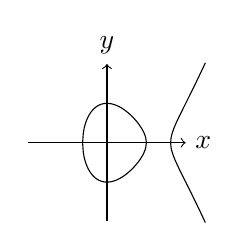
\begin{tikzpicture}
                \draw[->]
                    (-1,0) -- (1,0) node[right] {$x$};
                \draw[->]
                    (0,-1) -- (0,1) node[above] {$y$};
                \draw[scale=0.5,samples=100,domain=-0.618:1,variable=\x]
                    plot ({\x},{sqrt(abs(\x*\x*\x-2*\x*\x+1))});
                \draw[scale=0.5,samples=100,domain=1.618:2.5,variable=\x]
                    plot ({\x},{sqrt(abs(\x*\x*\x-2*\x*\x+1))});
                \draw[scale=0.5,samples=100,domain=-0.618:1,variable=\x]
                    plot ({\x},{-sqrt(abs(\x*\x*\x-2*\x*\x+1))});
                \draw[scale=0.5,samples=100,domain=1.618:2.5,variable=\x]
                    plot ({\x},{-sqrt(abs(\x*\x*\x-2*\x*\x+1))});
            \end{tikzpicture}
        \end{subfigure}
        \begin{subfigure}{0.25\textwidth}
            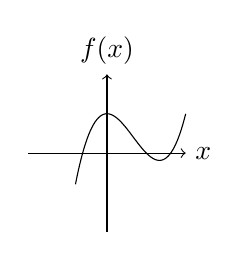
\begin{tikzpicture}
                \draw[->]
                    (-1,0) -- (1,0) node[right] {$x$};
                \draw[->]
                    (0,-1) -- (0,1) node[above] {$f(x)$};
                \draw[scale=0.5,domain=-0.8:2,samples=100,variable=\x]
                    plot ({\x},{\x*\x*\x-2*\x*\x+1});
            \end{tikzpicture}
        \end{subfigure}

        \medskip
        \begin{subfigure}{0.25\textwidth}
            \begin{tikzpicture}
                \draw[->]
                    (-1,0) -- (1,0) node[right] {$x$};
                \draw[->]
                    (0,-1) -- (0,1) node[above] {$y$};
                \draw[scale=0.5,samples=100,domain=1.678:2.5,variable=\x]
                    plot ({\x},{sqrt(abs(\x*\x*\x-1.5*\x*\x-0.5))});
                \draw[scale=0.5,samples=100,domain=1.678:2.5,variable=\x]
                    plot ({\x},{-sqrt(abs(\x*\x*\x-1.5*\x*\x-0.5))});
            \end{tikzpicture}
        \end{subfigure}
        \begin{subfigure}{0.25\textwidth}
            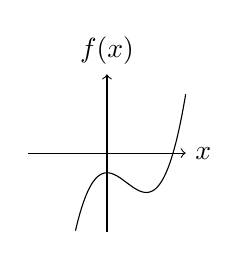
\begin{tikzpicture}
                \draw[->]
                    (-1,0) -- (1,0) node[right] {$x$};
                \draw[->]
                    (0,-1) -- (0,1) node[above] {$f(x)$};
                \draw[scale=0.5,domain=-0.8:2,samples=100,variable=\x]
                    plot ({\x},{\x*\x*\x-1.5*\x*\x-0.5});
            \end{tikzpicture}
        \end{subfigure}

        \medskip
        \begin{subfigure}{0.25\textwidth}
            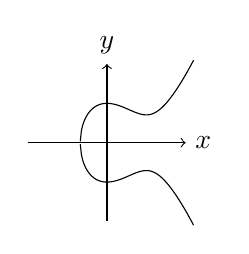
\begin{tikzpicture}
                \draw[->]
                    (-1,0) -- (1,0) node[right] {$x$};
                \draw[->]
                    (0,-1) -- (0,1) node[above] {$y$};
                \draw[scale=0.5,samples=100,domain=-0.678:2.2,variable=\x]
                    plot ({\x},{sqrt(abs(\x*\x*\x-1.5*\x*\x+1))});
                \draw[scale=0.5,samples=100,domain=-0.678:2.2,variable=\x]
                    plot ({\x},{-sqrt(abs(\x*\x*\x-1.5*\x*\x+1))});
            \end{tikzpicture}
        \end{subfigure}
        \begin{subfigure}{0.25\textwidth}
            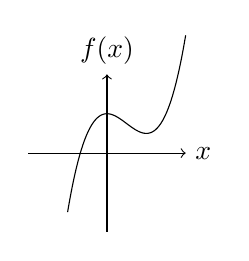
\begin{tikzpicture}
                \draw[->]
                    (-1,0) -- (1,0) node[right] {$x$};
                \draw[->]
                    (0,-1) -- (0,1) node[above] {$f(x)$};
                \draw[scale=0.5,samples=100,domain=-1:2,variable=\x]
                    plot ({\x},{\x*\x*\x-1.5*\x*\x+1});
            \end{tikzpicture}
        \end{subfigure}
    \end{figure}
\end{example}

\begin{theorem}[see Silverman, Chapter III]
    Let $\E$ be an elliptic curve over $K$. Then there exists an isomorphism (of
    projective varieties) from $\E$ to the projective curve defined by
    \begin{equation*}
        E : y^2 + a_1xy + a_3y = x^3 + a_2x^2 + a_4x + a_6
    \end{equation*}
    for some $a_i\in K$, mapping the given $K$-rational point to the point at
    infinity.
\end{theorem}

\begin{remark}
    To keep track of the indices for the Weierstrass equation, give $x$ weight
    2, $y$ weight 3, and $a_i$ weight $i$. The terms all have weight 6.
\end{remark}

\begin{example}
    Take $\E:y^2=x^4-1$ with point $P=(1,0)$.
    \begin{itemize}
        \item Let $x_2=x-1$, giving $y^2=x_2(x_2+2)(x_2^2+2x_2+2)$. (Move $P$ to
            the origin.)
        \item Let $x_3=1/x_2$, giving $(x_3^2y)^2=(1+2x_3)(1+2x_3+2x_3^2)$.
            (Move $P$ to infinity.)
        \item Let $y_2=yx_3^2$, giving $y_2^2=4x_3^3+6x_3^2+4x_3+1$. (Make monic
            in $y$.)
        \item Let $y_3=y_2/2$, giving $y_3^2=x_3^3+\frac{3}{2}x_3^2+x_3+\frac{1}{4}$.
            (Make monic in $x$.)
    \end{itemize}
    Note here we need $\ch K\ne2$. In fact this is a sloppy example, since the
    naive projectivization of the equation is singular. Instead one should
    use the equation $t^2=1-s^4$ at infinity, where $s=1/x$, $t=y/x^2$.
\end{example}

\begin{proposition}[see Silverman, Chapter III]
    ~
    \begin{enumerate}[label=(\roman*)]
        \item One can further simplify the Weierstrass equation to
            \begin{equation*}
                E : y^2 = x^3 + ax^2 + bx + c
            \end{equation*}
            when $\ch K\ne2$, and to
            \begin{equation*}
                E : y^2 = x^3 + Ax + B
            \end{equation*}
            when $\ch K\ne2,3$.

        \item Two curves given by generalized Weierstrass equations $E$ and $E'$
            are isomorphic over $K$ iff they are related by a change of
            variables of the form
            \begin{equation*}
                x=u^2x'+r,\quad y=u^3y'+u^2sx'+t
            \end{equation*}
            for some $u,r,s,t\in K$ with $u\ne0$.

        \item If $\ch K\ne2$, and $E:y^2=x^3+ax^2+bx+c$, then $E$ is
            non-singular iff the RHS cubic has no repeated roots, i.e. iff its
            discriminant is non-zero.
    \end{enumerate}
\end{proposition}

\begin{definition}
    Suppose $E/K$ is an elliptic curve given by a Weierstrass equation. Let
    $P,Q\in E(K)$. Define their \emph{sum} $P\oplus Q$ (or just $P+Q$) by the
    following process:
    \begin{figure}[htb]
        \centering
        \begin{tikzpicture}
            \draw[-] (-1.5,-0.9795) -- (2.5,1.039);
            \draw[-] (1.859,2) -- (1.859,-2);
            \node[circle,fill,inner sep=1pt,label=above left:$P$]
                at (-0.544,-0.497) {};
            \node[circle,fill,inner sep=1pt,label=$Q$]
                at (0.94,0.252) {};
            \node[circle,fill,inner sep=1pt,label=below right:$R$]
                at (1.859,0.716) {};
            \node[circle,fill,inner sep=1pt,label=right:$P\oplus Q$]
                at (1.859,-0.716) {};
            \draw[samples=100,domain=-0.618:1,variable=\x]
                plot ({\x},{sqrt(abs(\x*\x*\x-2*\x*\x+1))});
            \draw[samples=100,domain=1.618:3,variable=\x]
                plot ({\x},{sqrt(abs(\x*\x*\x-2*\x*\x+1))});
            \draw[samples=100,domain=-0.618:1,variable=\x]
                plot ({\x},{-sqrt(abs(\x*\x*\x-2*\x*\x+1))});
            \draw[samples=100,domain=1.618:3,variable=\x]
                plot ({\x},{-sqrt(abs(\x*\x*\x-2*\x*\x+1))});
        \end{tikzpicture}
    \end{figure}

    The line through $P$ and $Q$, or the tangent if $P=Q$, meets $E$ at exactly
    one other point $R$ when counting with multiplicity. Repeat the process with
    $\O$ and $R$, i.e. reflect $R$ across $y=0$, to obtain $P\oplus Q$.
\end{definition}

\begin{remark}
    If $P,Q\in E(K)$ then $P\oplus Q\in E(K)$. (If two roots of a cubic are
    rational then the third is too.) This gives a process to construct new
    rational points from old ones.
\end{remark}

\begin{theorem}
    The operation $\oplus$ makes $E(K)$ an abelian group with identity $\O$.
\end{theorem}

\begin{proof}
    See Silverman, Chapter III. See next section for the characteristic 0 case.
\end{proof}

\begin{remark}
    \begin{enumerate}[label=(\roman*)]
        \item If $P=(x_1,y_1)$, then $\ominus P=(x_1,-y_1-a_1x-a_3)$ for a
            generalized Weierstrass equation.

        \item If $F/K$ is a field extension, then $E(K)\subseteq E(F)$ is a
            subgroup.

        \item For $E:y^2=(x-a)(x-b)(x-c)$, the points where $y=0$ are precisely
            the points of order 2.
    \end{enumerate}
\end{remark}

\begin{example}
    The equation $y^2=(x-1)(x-2)(x-3)\mod p$, where $p\ne2$ is prime, has
    total number of solutions $N\equiv3\mod 4$. Indeed $E(\F_p)$ has a subgroup
    isomorphic to $C_2\times C_2$ given by the points of order 2 and the
    identity, so $4\mid\#E(\F_p)$, and removing the point at infinity gives
    $N=\#E(\F_p)-1$.
\end{example}

\begin{theorem}[Mordell 1922]
    Let $E/\Q$ be an elliptic curve. Then $E(\Q)$ is a finitely generated
    abelian group.
\end{theorem}

\begin{proof}
    See section 4.
\end{proof}

\begin{remark}
    So $E(\Q)\simeq\Delta\times\Z^r$ for some $r\ge0$ and finite group $\Delta$.
\end{remark}

\begin{definition}
    With $E(\Q)\simeq\Delta\times\Z^r$ as above $r$ is the \emph{rank} of
    $E/\Q$, and $\Delta$ the torsion subgroup of $E(\Q)$.
\end{definition}

\begin{remark}
    The result also holds over number fields, and for all abelian varieties
    (Mordell--Weil theorem).
\end{remark}

\begin{remark}
    To describe $E(\Q)$, one is happy with having generators for the group;
    finite data from which the points can be enumerated computationally. One
    cannot parametrize $E(\Q)$ like the conics: there are no non-constant
    $P(t),Q(t)\in\Q(t)$ satisfying the equation of an elliptic curve. (Otherwise
    we get a rational map $\P^1_\C\to E(\C)$ contradicting the Riemann--Hurwitz
    formula.)
\end{remark}

\begin{example}
    ~
    \begin{itemize}
        \item $E:y^2-y=x^3-x$ has
            $E(\Q)=\{\O,(0,0),(0,1),(1,0),(1,1)\}\simeq C_5$.

        \item $E:y^2+y=x^3-x$ has $E(\Q)\simeq\Z$ generated by $(0,0)$.

        \item $E:y^2+y=x^3+x-2x$ has $E(\Q)\simeq\Z^2$ generated by $(0,0)$ and
            $(1,0)$.

        \item $E:y^2=x^3-2x$ has $E(\Q)\simeq C_2\times\Z$ generated by $(0,0)$
            and $(-1,1)$ respectively.

        \item $E:y^2=x^3+877x$ has $E(\Q)\simeq C_2\times\Z$ generated by $(0,0)$
            and $(\textit{a horrid mess})$ respectively.
    \end{itemize}
\end{example}

\subsection*{Exercise Sheet 1}

\begin{enumerate}
    \item[+1.] Let $E$ be the elliptic curve given by
        \begin{equation*}
            y^2-y = x^3-x^2.
        \end{equation*}
        Verify that the point $P=(0,0)$ has order 5.

        \begin{proof}[Solution]
            The tangent at $P$ is $y=0$, which intersects $E$ when $x^3-x^2=0$.
            The third point is then $(1,0)$, and the line through $(1,0)$ and
            $\O$ intersects $E$ again at $(1,1)$. Hence $2\cdot P=(1,1)$.

            The tangent at $(1,1)$ is $y=x$, which intersects $E$ when
            $x^2-x=x^3-x^2$. The third point is then $(0,0)$, and the line
            through $(0,0)$ and $\O$ intersects $E$ again at $(0,1)$. Hence
            $4\cdot P=(0,1)$.

            The line through $P$ and $(0,1)$ is $x=0$, which meets $E$ at the
            point $\O$ at infinity. Hence $5\cdot P=\O$, so $P$ has order 5.
        \end{proof}

    \item[+2.] Let $E/\Q$ be an elliptic curve that has a rational point of order
        3. Show that $E$ is isomorphic to one of the form
        \begin{equation*}
            y^2 = x^3 + (ax-b)^2.
        \end{equation*}
        (\textit{Hint: you may find it helpful to show that a point $P$ has
        order 3 if and only if the tangent line to $E$ through $P$ intersects
        $E$ at $P$ with multiplicity 3.})

        \begin{proof}[Solution]
            We have $3\cdot P=\O$ iff the tangent line at $P$ intersects $E$
            at $P$ only. By Proposition 1(i), we may assume $E$ has an equation
            of the form $y^2=x^3+px^2+qx+r$, and by translation we may assume
            the rational point $P$ of order 3 is of the form $(0,\beta)$. If
            $\beta=0$ then $r=0$ and $q\ne0$ by non-singularity, so the tangent
            line at $P$ is the $y$-axis, whose intersections with $E$ are given
            by the cubic equation $x^3+px^2+qx=0$. This has at least two
            distinct roots, since $q\ne0$, contradicting the fact that $P$ is
            the only intersection of the tangent line with $E$. Hence
            $\beta\ne0$, so the tangent line at $P$ is
            \begin{equation*}
                y = \beta + \frac{q}{2\beta}x,
            \end{equation*}
            which intersects $E$ when
            \begin{align*}
                &\bigl(\beta+\frac{q}{2\beta}x\bigr)^2 = x^3 + px^2 + qx + r \\
                &\iff x^3 + \bigl(p-\frac{q^2}{4\beta^2}\bigr)x^2 + r - \beta^2
                    = 0.
            \end{align*}
            Then since $3\cdot P=\O$ this cubic has only the one root at $x=0$,
            meaning
            \begin{equation*}
                p - \frac{q^2}{4\beta^2} = r-\beta^2 = 0,
            \end{equation*}
            so
            \begin{align*}
                E : y^2
                    &= x^3 + \frac{q^2}{4\beta^2}x^2 + qx + \beta^2 \\
                    &= x^3 + \bigl(\frac{q}{2\beta}x+\beta\bigr)^2,
            \end{align*}
            which is of the desired form with $a=\frac{q}{2\beta}$ and
            $b=-\beta$.
        \end{proof}

    \item[3.] Determine the group $E(\F_3)$ for the elliptic curves
        \begin{equation*}
            E:y^2=x^3-x  \qquad \text{and} \qquad E:y^2=x^3+x.
        \end{equation*}

        \begin{proof}[Solution]
            For $E:y^2=x^3-x$ the polynomial $x^3-x$ vanishes on $\F_3$, so the
            points (apart from $\O$) are $\{(x,0):x\in\F_3\}$. All have order 2
            since $y=0$, so $E(\F_3)\simeq C_2\times C_2$.

            For $E:y^2=x^3+x$ the points (apart from $\O$) are
            $\{(0,0),(2,1),(2,2)\}$. Since $(2,1)$ and $(2,2)$ do not have order
            2, having $y\ne0$, we have $E(\F_3)\simeq C_4$.
        \end{proof}

    \item[4.] Let $E$ and $E'$ be two elliptic curves over a field $K$ given by
        Weierstrass equations. Show that if the elliptic curves $E$ and $E'$ are
        isomorphic, then so are the groups $E(K)$ and $E'(K)$.

        \begin{proof}[Solution]
            By Proposition 1(ii) we may assume $E$ and $E'$ are related by a
            linear change of coordinates. Now a $K$-linear change of coordinates
            preserves $K$-rational points, lines, incidence, and tangency, and
            therefore preserves the definition of the group law on $E(K)$. Hence
            it gives a group isomorphism $E(K)\simeq E'(K)$.
        \end{proof}

    \item[!5.] Prove that for every positive integer $N\equiv5\mod8$, the
        elliptic curve
        \begin{equation*}
            y^2 = x^3-N^2x
        \end{equation*}
        has a rational point with a non-zero $y$-coordinate.
\end{enumerate}

\section{Elliptic Curves / $\C$}

Recall that for an elliptic curve $E$ we defined an operation on rational points
geometrically via intersections of lines with $E$. Now an elliptic curve $E/\C$
is supposed to be a torus (a genus 1 Riemann surface), and the standard
construction of a complex torus as $\C/\Lambda$ for a lattice $\Lambda$ has an
obvious group structure as a quotient of $(\C,+)$. How does this relate to the
group structure given by line intersections?

\begin{proposition}[Recall from complex analysis]
    A function $f:\C\to\C$ is meromorphic iff at
    every $a\in\C$ it has a Laurent series expression
    \begin{equation*}
        f(z) = \sum_{n=n_0}^\infty c_n(z-a)^n
    \end{equation*}
    where $n_0\in\Z$ and $c_{n_0}\ne0$ unless $f(z)\equiv0$. We write
    \begin{equation*}
        \ord_af = n_0 \quad \text{and} \quad \res_af=c_{-1}.
    \end{equation*}
\end{proposition}

\begin{definition}
    A \emph{lattice} $\Lambda\subseteq\C$ is a discrete rank 2 subgroup of
    $(\C,+)$. Say
    \begin{equation*}
        \Lambda = \Z\omega_1\oplus\Z\omega_2.
    \end{equation*}
    The parallelogram spanned by $\omega_1$ and $\omega_2$ is the
    \emph{fundamental parallelogram}, denoted $\Pi$.
\end{definition}

\textit{Idea:} Curves are essentially degree 1 transcendental extensions of
$\C$, and the Riemann surface $\C/\Lambda$ has a field of meromorphic functions,
so we check if that field has transcendence degree 1 over $\C$.

\begin{definition}
    An \emph{elliptic function} (w.r.t. $\Lambda$) is a meromorphic function $f$
    on $\C$ such that $f(z+w)=f(z)$ for all $w\in\Lambda$. In other words, a
    doubly-periodic meromorphic function.
\end{definition}

\begin{remark}
    These are precisely the meromorphic functions on the Riemann surface
    $X=\C/\Lambda$. They form a field, since we allow poles, denoted $\C(X)$.
\end{remark}

\begin{lemma}
    Suppose $f$ is a non-zero elliptic function.
    \begin{enumerate}[label=(\roman*)]
        \item If $f$ is analytic, then $f$ is constant.
        \item We have $\ord_af\ne0$ at only finitely many $a\in\C/\Lambda$.
        \item $\sum_{a\in\C/\Lambda}\res_af=0$.
        \item $\sum_{a\in\C/\Lambda}\ord_af=0$.
        \item $\sum_{a\in\C/\Lambda}\ord_af\cdot a\in\Lambda$.
    \end{enumerate}
\end{lemma}

\begin{proof}
    \begin{enumerate}[label=(\roman*)]
        \item If $f$ is analytic then $f$ is continuous, and hence bounded on
            $\Pi$ since $\Pi$ is compact. By periodicity $f$ is bounded on $\C$,
            and hence constant by Liouville's theorem.

        \item Otherwise, we have an accumulation point in $\Pi$ either of zeros
            or of poles. In the former case $f=0$ by the identity theorem, and
            in the latter case the limit point is an essential singularity. (One
            can also reduce to only one of these cases by considering $1/f$.)

        \item After translating $\Pi$ by some amount we can assume no zeros or
            poles like on $\partial\Pi$, since there are only finitely many.
            Then
            \begin{equation*}
                \sum_{a\in\C/\Lambda}\res_af
                    = \frac{1}{2\pi i}\oint_{\partial\Pi}f(z)dz
            \end{equation*}
            by the residue theorem. The integral splits up into four parts
            \begin{equation*}
                \oint_{\partial\Pi}
                    = \left[\int_0^{\omega_1}
                        + \int_{\omega_1+\omega_2}^{\omega_2}\right]
                    + \left[\int_{\omega_2}^0
                        + \int_{\omega_1}^{\omega_1+\omega_2}\right],
            \end{equation*}
            but since the integrand is doubly periodic we have
            \begin{equation*}
                \int_0^{\omega_1} = -\int_{\omega_1+\omega_2}^{\omega_2}
                \quad \text{and} \quad
                \int_{\omega_2}^0 = -\int_{\omega_1}^{\omega_1+\omega_2},
            \end{equation*}
            so the result is zero.

        \item Apply (iii) to $f'(z)/f(z)$, whose residues are the orders of
            $f(z)$ by local Taylor expansion.

        \item Exercise. (Use $zf'(z)/f(z)$.)
    \end{enumerate}
\end{proof}

We are prompted to ask, are there any non-constant elliptic functions? From
above they must have at least two poles, or a double pole. The answer is yes,
via (almost) the most obvious construction.

\begin{definition}
    The \emph{Weierstrass $\wp$-function} (w.r.t. $\Lambda$) is given by
    \begin{equation*}
        \wp(z) = \wp_\Lambda(z)
            = \frac{1}{z^2} + \sum_{w\in\Lambda\setminus\{0\}}
                \left(\frac{1}{(z-w)^2}-\frac{1}{w^2}\right).
    \end{equation*}
\end{definition}

\begin{exercise}
    The sum $\sum_{w\in\Lambda\setminus\{0\}}\frac{1}{|w|^\alpha}$ converges iff
    $\alpha>2$.
\end{exercise}

\begin{proposition}
    The expression for $\wp(z)$ converges locally uniformly to an elliptic
    function analytic on $\C\setminus\Lambda$ with doubles poles on $\Lambda$.
\end{proposition}

\begin{proof}
    If $2|z|<|w|$, then
    \begin{equation*}
        \left|\frac{1}{(z-w)^2}-\frac{1}{w^2}\right|
            = \left|\frac{z(2w-z)}{w^2(z-w)^2}\right|
            \le \frac{\frac{5}{2}|zw|}{\frac{1}{4}|w|^4}
            = 10\frac{|z|}{|w|^3}.
    \end{equation*}
    Hence
    \begin{equation*}
        \sum_{|w|>2|z|}\left|\frac{1}{(z-w)^2}-\frac{1}{w^2}\right|
        \le 10|z|\sum_{w\in\Lambda\setminus\{0\}}\frac{1}{|w|^3},
    \end{equation*}
    which is a finite constant multiple of $|z|$ by the exercise above.
    Therefore the series converges locally uniformly absolutely on
    $\C\setminus\Lambda$, and the limit is an analytic function on
    $\C\setminus\Lambda$. Clearly it has double poles on $\Lambda$. To see that
    $\wp$ is elliptic, note that
    \begin{equation*}
        \wp'(z) = -2\sum_{w\in\Lambda}\frac{1}{(z-w)^3}
    \end{equation*}
    which is clearly elliptic, so $\wp(z+w)-\wp(z)=C(w)$ is a constant depending
    on $w\in\Lambda$. But we can see that $\wp(z)=\wp(-z)$ by definition, so
    $\wp(-w/2)=\wp(w/2)=\wp(-w/2+w)$, so $C(w)=0$.
\end{proof}

\begin{lemma}
    ~
    \begin{enumerate}[label=(\roman*)]
        \item $\wp(z)$ is even.
        \item $\wp'(z)$ is odd.
        \item $\wp(z)-\wp(\alpha)$ has a double pole at $0+\Lambda$, simple
            zeros at $\pm\alpha+\Lambda$ (or a double zero if
            $2\alpha\in\Lambda$), and no other zeros or poles.
    \end{enumerate}
\end{lemma}

\begin{proof}
    (i) was noted above. (ii) follows immediately. For (iii) the statement about
    poles is clear, and the statement about zeros follows by counting using
    Lemma 6(iv).
\end{proof}

\begin{theorem}
    Let $\Lambda\subseteq\C$ be a lattice, and set $X=\C/\Lambda$.
    \begin{enumerate}[label=(\roman*)]
        \item $\C(X)=\C(\wp(z),\wp'(z))$.
        \item Every even elliptic function lies in $\C(\wp(z))$.
    \end{enumerate}
\end{theorem}

\begin{proof}
    For (ii), suppose an even elliptic function $f(z)$ has zeros/poles away from
    $\Lambda$ at $\pm z_i\notin\Lambda$, with $\ord_{\pm z_i}f=n_i$. (If
    $2z_i\in\Lambda$ take $n_i=\frac{1}{2}\ord_{z_i}f$.) Consider
    \begin{equation*}
        \tilde f(z)=\prod_i(\wp(z)-\wp(z_i))^{n_i} \in \C(\wp(z)).
    \end{equation*}
    Then $f(z)/\tilde f(z)$ has no zeros/poles except possibly on $\Lambda$ by
    Lemma 8(iii). By Lemma 6(iv) then $f(z)/\tilde f(z)$ has no zeros/poles at
    all, and hence is constant. Therefore $f(z)\in\C(\wp(z))$. For (i), write an
    arbitrary elliptic function $f(z)$ as a sum
    \begin{equation*}
        f(z) = \frac{f(z)+f(-z)}{2} + \frac{f(z)-f(-z)}{2}
    \end{equation*}
    of an even and an odd elliptic function. Since an odd function is an even
    multiple of the odd function $\wp'(z)$, we are done by (ii). In fact we see
    that $\C(\wp(z),\wp'(z))$ is a quadratic extension of $\C(\wp(z))$.
\end{proof}

\begin{definition}
    We define
    \begin{equation*}
        G_{2k} = G_{2k}(\Lambda)
            = \sum_{w\in\Lambda\setminus\{0\}}\frac{1}{w^{2k}} \in \C
    \end{equation*}
    for $k\ge2$. This is known as the \emph{Eisenstein series} of weight $2k$.
\end{definition}

\begin{remark}
    This is a two-dimensional version of the special values $\zeta(2k)$ for
    $k\ge1$.
\end{remark}

\begin{lemma}
    The Taylor series expansion around $z=0$ of $\wp(z)$ is
    \begin{equation*}
        \wp(z) = \frac{1}{z^2} + \sum_{k=1}^\infty(2k+1)G_{2k+2}z^{2k}.
    \end{equation*}
\end{lemma}

\begin{proof}
    We have
    \begin{equation*}
        \frac{1}{(z-w)^2} - \frac{1}{w^2}
            = \frac{1}{w^2}\cdot\frac{1}{\bigl(1-\frac{z}{w}\bigr)^2-1}
            = \frac{1}{w^2}\sum_{k=1}^\infty\frac{2k+1}{w^{2k}}z^{2k}.
    \end{equation*}
    Summing over $w$ gives the result.
\end{proof}

\begin{lemma}
    We have the equation
    \begin{equation*}
        \frac{1}{4}\wp'(z)^2 = \wp(z)^3 - 15G_4\wp(z) - 35G_6.
    \end{equation*}
\end{lemma}

\begin{proof}
    From the Taylor expansions
    \begin{align*}
        \wp(z) &= \frac{1}{z^2} + 3G_4z^2 + 5G_6z^4 + \cdots \\
        \wp(z)^3 &= \frac{1}{z^6} + \frac{9G_4}{z^2} + 15G_6 + \cdots \\
        \frac{1}{4}\wp'(z)^2 &= \frac{1}{z^6} - \frac{6G_4}{z^2} - 20G_6 + \cdots
    \end{align*}
    we see that the difference between the two sides of the equation is analytic
    and vanishes at the origin, whence it is identically zero.
\end{proof}

\begin{theorem}
    Let $\Lambda\subseteq\C$ be a lattice. Then
    \begin{equation*}
        E_\Lambda : y^2 = x^3 - 15G_4x - 35G_6
    \end{equation*}
    defines an elliptic curve over $\C$, i.e. it is non-singular, and
    \begin{equation*}
        \varphi(z) = (\wp(z),\frac{1}{2}\wp'(z)) \qquad \wp(0)=\O
    \end{equation*}
    is an isomorphism of groups $\C/\Lambda\to E_\Lambda(\C)$.
\end{theorem}

\begin{proof}
    \begin{itemize}
        \item $\varphi$ is well-defined by Lemma 11 and periodicity of $\wp$.

        \item $\varphi$ is bijective: if $(x_0,y_0)\in E_\Lambda(\C)$, then
            $\wp(z)-x_0$ has one double pole, and therefore two zeros
            $\pm\alpha$, giving
            \begin{equation*}
                \{\varphi(\alpha),\varphi(-\alpha)\} = \{(x_0,y_0),(x_0,-y_0)\}.
            \end{equation*}
            Hence $\varphi$ is a bijection.

        \item $E_\Lambda$ is non-singular: as $\wp'(z)$ is odd, it vanishes at
            the three points $\tau$ of order 2 in $\C/\Lambda$, and hence the
            roots of the cubic in $x$ are the images $\wp(\omega_1/2)$,
            $\wp(\omega_2/2)$, $\wp((\omega_1+\omega_2)/2)$ of these points.
            These roots are distinct, since $\wp(z)-\wp(\tau)$ has a double root
            at $\tau$ and hence no other zeros.

        \item $\varphi$ is a group homomorphism:
            \begin{itemize}
                \item $\varphi(0)=\O$.
                \item $\varphi(-\alpha)$ and $\varphi(\alpha)$ lie on a vertical
                    line since $\wp(z)$ is even.

                \item Suppose $P_1\oplus P_2=\ominus P_3$, with $\{P_i\}$ lying
                    on the line
                    \begin{equation*}
                        \lambda y + \mu x + \nu = 0.
                    \end{equation*}
                    Writing $P_i=\varphi(\alpha_i)$, the elliptic function
                    $\frac{\lambda}{2}\wp'(z)+\mu\wp(z)+\nu$ vanishes at each
                    $\alpha_i$, and has a triple pole on $\Lambda$. By Lemma
                    6(v) we therefore have $\alpha_1+\alpha_2+\alpha_3=0$.
            \end{itemize}
    \end{itemize}
\end{proof}

\begin{remark}
    The result shows that $(E_\Lambda(\C),\oplus)$ is indeed a group.
\end{remark}

\begin{theorem}[Uniformization Theorem]
    Every elliptic curve over $\C$ is isomorphic to $E_\Lambda$ for some
    $\Lambda$.
\end{theorem}

\begin{proof}
    Beyond the scope of the course.
\end{proof}

\begin{corollary}
    Let $K$ be a number field, and $E/K$ an elliptic curve. Then
    $E(K)[n]\le\Z/n\Z\oplus\Z/n\Z$.
\end{corollary}
Here $A[n]=\{a\in A:na=0\}$ denotes the $n$-torsion subgroup of an abelian group
$A$.

\begin{proof}
    By the uniformization theorem we have
    $E(K)\le E(\C)\simeq E_\Lambda(\C)\simeq\C/\Lambda$ for some $\Lambda$. But
    by inspection $(\C/\Lambda)[n]\simeq\Z/n\Z\oplus\Z/n\Z$.
\end{proof}

\begin{corollary}
    Let $E:y^2+a_1xy+a_3y=x^3+a_2x^2+a_4x+a_6$ be an elliptic curve over a field
    of characteristic 0. Then $(E(K),\oplus)$ is a group.
\end{corollary}

Note that $K$ may have cardinality too large to embed into $\C$.

\begin{proof}
    This is an example of the ``Lefschetz principle''. All group axioms apart
    from associativity are easy. Suppose $P_i=(x_i,y_i)\in E(K)$ for $i=1,2,3$.
    Define the field $F=\Q(a_1,a_2,a_3,a_4,a_6,x_1,y_1,x_2,y_2,x_3,y_3)$, which
    embeds into $\C$ as a finitely generated $\Q$-extension. We may then view
    $E$ over $\C$ via this embedding, and $P_i\in E(F)\le E(\C)$ where
    $(P_1\oplus P_2)\oplus P_3=P_1\oplus(P_2\oplus P_3)$ by the previous result.
\end{proof}

\subsection*{Exercise Sheet 2}

\begin{enumerate}
    \item[+1.]
        Let $E/\C$ be an elliptic curve given by
        \begin{equation*}
            y^2 = x^3 + Ax + B,
        \end{equation*}
        and let $m\ge1$ be an integer. Use the uniformization theorem to show
        that there are rational functions $f,g$ such that for every
        $P=(x_1,y_1)\in E(\C)$, the point $mP$ is given by $(f(x_1),y_1g(x_1))$.

        \begin{proof}[Solution]
            By the uniformization theorem $E\simeq E_\Lambda$ for some $\Lambda$,
            and by Proposition 2(ii) there is an isomorphism given by a linear
            change of coordinates of the form
            \begin{equation*}
                x=u^2x'+r,\quad y=u^3y'+u^2sx'+t.
            \end{equation*}
            Since $E_\Lambda$ has no $xy$ and no $y$ term we have $s=t=0$, and
            so this change of coordinates preserves functions of the desired
            form $(f(x),yg(x))$. Hence we may assume $E=E_\Lambda$, where there
            is the group isomorphism $\C/\Lambda\to E_\Lambda(\C)$ given by
            $z+\Lambda\mapsto(\wp(z),\frac{1}{2}\wp'(z))$. Then if
            $(x_1,y_1)=(\wp(z),\frac{1}{2}\wp'(z))$, the coordinates of $mP$ are
            $(\wp(mz),\frac{1}{2}\wp'(mz))$, and it suffices to note that
            $\wp(mz)$ and $\wp'(mz)/\wp'(z)$ are even elliptic functions, hence
            given by rational functions $f,g$ of $\wp(z)$.
        \end{proof}

    \item[+2.] Let $\Lambda$ be a lattice in $\C$ and $f$ an elliptic function
        with respect to $\Lambda$. Prove that
        $\sum_{z\in\C/\Lambda}(z\cdot\ord_zf)$ is an element of $\Lambda$.
        (\textit{Hint: Integrate $\frac{zf'(z)}{z}$ over the boundary of the
        fundamental parallelogram and don't be afraid of logs.})

        \begin{proof}[Solution]
            Assuming $f$ is non-zero it has finitely many zeros/poles, so we
            may translate it so that none lie on the boundary of the fundamental
            parallelogram $\Pi$. Then by the residue theorem
            \begin{align*}
                \frac{1}{2\pi i}\oint_{\partial\Pi}\frac{zf'(z)}{f(z)}dz
                    = \sum_{a\in\Pi}\res_a\frac{zf'(z)}{f(z)}
                    = \sum_{a\in\Pi}\biggl(a\cdot\res_a\frac{f'(z)}{f(z)}\biggr)
                    = \sum_{a\in\Pi}(a\cdot\ord_af).
            \end{align*}
            Now if $\Lambda$ is generated by $\omega_1,\omega_2$, then
            \begin{align*}
                \oint_{\partial\Pi}\frac{zf'(z)}{f(z)}dz
                    &= \int_0^{\omega_1}\biggl[\frac{zf'(z)}{f(z)}
                        - \frac{(z+\omega_2)f'(z+\omega_2)}{f(z+\omega_2)}
                        \biggr]dz \\
                    &\qquad + \int_0^{\omega_2}\biggl[
                        \frac{(z+\omega_1)f'(z+\omega_1)}{f(z+\omega_1)}
                        - \frac{zf'(z)}{f(z)}\biggr]dz \\
                    &= -\omega_2\int_0^{\omega_1}\frac{f'(z)}{f(z)}dz
                        + \omega_1\int_0^{\omega_2}\frac{f'(z)}{f(z)}dz.
            \end{align*}
            But the integral
            \begin{equation*}
                \int_0^{\omega_i}\frac{f'(z)}{f(z)}dz
                    = \int_0^{\omega_i}d\log f(z)
            \end{equation*}
            is the increment of the analytic continuation of the logarithm
            along $f([0,\omega_i])$; a loop based at $f(\omega_i)=f(0)$. This
            is an integer multiple of $2\pi i$, so
            $\frac{1}{2\pi i}\oint_{\partial\Pi}\frac{zf'(z)}{f(z)}dz
            \in\Z\omega_2+\Z\omega_1=\Lambda$.
        \end{proof}

    \item[3.] Let $E/K$ be an elliptic curve over a field of characteristic
        zero. Prove that
        \begin{equation*}
            E(\bar K)[n] \simeq \Z/n\Z\oplus\Z/n\Z.
        \end{equation*}

        \begin{proof}[Solution]
            By a change of coordinates we may assume $E:y^2=x^3+Ax+B$ for some
            $A,B\in K$. The map $P\mapsto nP$ on $E(L)$ for any $L/K$ is given
            by $(x,y)\mapsto(p(x,y),q(x,y))$ for some $p,q\in K(x,y)$. Let
            $F/\Q$ be the extension generated by $A$, $B$, and the coefficients
            of $p$ and $q$. Then $F$ embeds into $\C$, and we may view $E/F$.
            From exercise 1 we have that $p(x,y)$ and $q(x,y)/y$ lie in
            $F(x,y)\cap\C(x)=F(x)$; say $p(x,y)=P_1(x)/P_2(x)$ and
            $q(x,y)=yQ_1(x)/Q_2(x)$ where $P_i,Q_i\in F[x]$. Then
            \begin{align*}
                E(\bar K)[n] = \{(x,y)\in E(\bar K)
                    : Q_2(x)=0,y=1/(Q_1(x)P_2(x))\}\cup\{\O\}
            \end{align*}
            is finite since $Q_2(x)$ has finitely many roots, so we may assume
            $F$ also contains the coordinates of all the points in
            $E(\bar K)[n]$, meaning $E(\bar F)[n]=E(\bar K)[n]$. Now
            \begin{equation*}
                E(\C)[n] = \{(x,y)\in E(\C)
                    : Q_2(x)=0,y=1/(Q_1(x)P_2(x))\}\cup\{\O\}
            \end{equation*}
            consists of points whose coordinates are algebraic over $F$, so
            since $\bar F$ embeds into $\C$ we must have
            $E(\bar F)[n]\simeq E(\C)[n]$. Hence
            \begin{equation*}
                E(\bar K)[n] = E(\bar F)[n] \simeq E(\C)[n]
                    \simeq \Z/n\Z\oplus\Z/n\Z
            \end{equation*}
            by the uniformization theorem.
        \end{proof}

    \item[4.] Let $E$ be an elliptic curve over $\F_p$ given by a Weierstrass
        equation. Prove that the operation $\oplus$ is associative.
        (\textit{Hint: Write $E$ as the reduction mod $p$ of a suitable
        elliptic curve with coefficients in $\Z_p$. You'll need Hensel's Lemma
        to lift points from $\F_p$ to $\Z_p$.})

        \begin{proof}[Solution]
            Firstly, note that the associativity equation
            $P\oplus(Q\oplus R)=(P\oplus Q)\oplus R$ for an elliptic curve is
            easily seen to be true in the following cases:
            \begin{itemize}
                \item If $P=\O$, $Q=\O$, or $R=\O$.
                \item If $P\oplus(Q\oplus R)=\O$ or $(P\oplus Q)\oplus R=\O$,
                    since these both happen iff $P,Q,R$ are collinear.
                \item If $P\oplus Q=\O$ or $Q\oplus R=\O$, since
                    $(-P)\oplus(P\oplus Q)=Q$: the points $P,Q,-(P\oplus Q)$ are
                    the intersections of a line with $E$, so the reflections
                    $-P,-Q,P\oplus Q$ are also. (For a Weierstrass equation
                    negation $(x,y)\mapsto(x,-y-a_1x-a_3)$ is linear and so
                    sends lines to lines.)
            \end{itemize}
            Now suppose
            \begin{equation*}
                y^2 + a_1xy + a_3y = x^3 + a_2x^2 + a_4x + a_6
            \end{equation*}
            is an equation over $\Z_p$ reducing to $E$ modulo $p$ which defines
            an elliptic curve $\tilde E/\Q_p$. One exists by completing the
            square and applying Proposition 2(iii); the discriminant cannot
            vanish for the infinitely many possible lifts of the coefficients.
            Since $\Q_p$ embeds into $\C$, we see that $\oplus$ is associative
            on $\tilde E(\Q_p)$ by the uniformization theorem.

            If $P\in\tilde E(\Z_p)$, write $\bar P\in E(\F_p)$ for the reduction
            modulo $p$. Since $E$ is non-singular, for every point in $E(\F_p)$
            one coordinate when fixed leaves the other as a simple root of the
            defining equation. By Hensel's lemma simple roots can be lifted to
            $\Z_p$, so all points of $E(\F_p)$ are of the form $\bar P$.

            \textbf{Claim:} If $P,Q\in\tilde E(\Z_p)$ with
            $\bar P\oplus\bar Q\ne\O$, then $P\oplus Q\in\tilde E(\Z_p)$ and
            $\overline{P\oplus Q}=\bar P\oplus\bar Q$.

            Since we dealt with the case of vanishing sums earlier, this proves
            associativity on $E(\F_p)$:
            \begin{equation*}
                \bar P\oplus(\bar Q\oplus\bar R)
                    = \bar P\oplus\overline{Q\oplus R}
                    = \overline{P\oplus Q\oplus R}
                    = \overline{P\oplus Q}\oplus\bar R
                    = (\bar P\oplus\bar Q)\oplus\bar R.
            \end{equation*}

            \textbf{Proof of claim:} Suppose $P=(x_1,y_1)$, $Q=(x_2,y_2)$, and
            $P\oplus Q=(x_3,y_3)$. Write $s=\frac{y_2-y_1}{x_2-x_1}\in\Z_p$,
            where $x_2-x_1$ is invertible in $\Z_p$ since
            $\bar P\oplus\bar Q\ne\O$. We have a monic cubic
            \begin{equation*}
                (y_1+s(x-x_1))^2 + (a_1x+a_3)(y_1+s(x-x_1))
                    = x^3 + a_2x^2 + a_4x + a_6
            \end{equation*}
            in $x$ over $\Z_p$, whose roots in $\Q_p$ are $x_1,x_2,x_3$, and
            whose roots upon reduction to $\F_p$ are the $x$-coordinates of
            $\bar P,\bar Q,\bar P\oplus\bar Q$. Factoring out $(x-x_1)(x-x_2)$
            we see that $x_3\in\Z_p$, since the equation is monic, and reducing
            to $\F_p$ we see that $x_3$ lifts the $x$-coordinate of
            $\bar P\oplus\bar Q$. Similarly, factoring out the root
            $y_1+s(x_1-x_3)$ of the monic quadratic
            \begin{equation*}
                y^2 + a_1x_3y + a_3y = x_3^3 + a_2x_3^2 + a_4x_3 + a_6
            \end{equation*}
            in $y$ over $\Z_p$, we see that $y_3\in\Z_p$ lifts the
            $y$-coordinate of $\bar P\oplus\bar Q$.
        \end{proof}

    \item[!5.] Fix an elliptic curve $E/\Q$ given by $y^2=x^3+Ax+B$ and consider
        the family of its ``quadratic twists'',
        \begin{equation*}
            d\cdot y^2=x^3+Ax+B,
        \end{equation*}
        where $d$ runs over all square-free integers (ordered by absolute
        value). Show that 50\% of the elliptic curves in this family have an
        infinite number of rational points.
\end{enumerate}

\section{Heights}

\begin{definition}
    For $\alpha=p/q\in\Q$ with $p$ and $q$ coprime, define the \emph{height} of
    $\alpha$
    \begin{equation*}
        H(\alpha) = H_\Q(\alpha) = \max\{|p|,|q|\},
    \end{equation*}
    and the \emph{logarithmic height} of $\alpha$
    \begin{equation*}
        h(\alpha) = \log H(\alpha).
    \end{equation*}
\end{definition}

\begin{notation}
    For a rational function $f(x)=P(x)/Q(x)\in K(x)$ over a field $K$ where
    $P(x),Q(x)\in K[x]$ have no common factor, we define the degree of $f$ to be
    $\max\{\deg P,\deg Q\}$.
\end{notation}

\begin{proposition}
    ~
    \begin{enumerate}[label=(\roman*)]
        \item $h(\alpha)\ge0$ for all $\alpha\in\Q$.

        \item $h(\alpha)=0$ iff $\alpha\in\{0,1,-1\}$.

        \item $h(\alpha^d)=d\cdot h(\alpha)$ for each $d\ge1$.

        \item If $f(x)=(a_nx^n+\cdots+a_0)/(b_mx^m+\cdots+b_0)\in\Q(x)$ has
            degree $d$, then $h(f(\alpha))=d\cdot h(\alpha)+O(1)$, i.e. there is
            a constant $c$ such that
            \begin{equation*}
                d\cdot h(\alpha) - c \le h(f(\alpha)) \le d\cdot h(\alpha) + c
            \end{equation*}
            for all $\alpha\in\Q$.

        \item The set $\{\alpha\in\Q:h(\alpha)<c\}$ is finite for each $c>0$.
    \end{enumerate}
\end{proposition}

\begin{proof}
    All except (iv) are clear. For (iv), we may assume without loss of
    generality that $n\ge m$, otherwise considering $1/f(x)$, and that
    $a_i,b_j\in\Z$. Write
    \begin{equation*}
        f(S/T)
            = \frac{a_nS^n+\cdots+a_0T^n}{(b_mS^m+\cdots+b_0T^m)T^{n-m}}
            = \frac{A(S,T)}{B(S,T)},
    \end{equation*}
    with $A(S,1)$ and $B(S,1)$ coprime in $\Q[S]$. Then for $\alpha=p/q$, we
    have
    \begin{equation*}
        |a_np^n+\cdots+a_0q^n|
            \le (n+1)\max\{|a_i|\}\max\{|p|,|q|\}^n
    \end{equation*}
    and
    \begin{equation*}
        |(b_mp^m+\cdots+b_0q^m)q^{n-m}|
            \le (m+1)\max\{|b_j|\}\max\{|p|,|q|\}^n,
    \end{equation*}
    so $H(f(\alpha))\le c_1H(\alpha)^n$ where
    $c_1=(n+1)\max(\{|a_i|\}\cup\{|b_j|\})$. On the other hand, since $A(S,1)$
    and $B(S,1)$ are coprime in $\Q[S]$ we have some $\phi(S),\psi(S)\in\Z[S]$
    with
    \begin{equation*}
        A(S,1)\phi(S)+B(S,1)\psi(S) = d_1\in\Z_{>0}.
    \end{equation*}
    By homogenizing terms, we get some
    $\tilde\phi(S,T),\tilde\psi(S,T)\in\Z[S,T]$ homogeneous of degree $N-n$ with
    \begin{equation*}
        A(S,T)\tilde\phi(S,T) + B(S,T)\tilde\psi(S,T) = d_1T^N
    \end{equation*}
    for a sufficiently large $N>n$. We also have that $A(1,T)$ and $B(1,T)$ are
    coprime in $\Q[T]$, and so for $N$ large enough we also get
    $\tilde\phi'(S,T),\tilde\psi'(S,T)\in\Z[S,T]$ homogeneous of degree $N-n$
    with
    \begin{equation*}
        A(S,T)\tilde\phi'(S,T) + B(S,T)\tilde\psi'(S,T) = d_2S^N,
    \end{equation*}
    where $d_2\in\Z_{>0}$. Now $\gcd\{A(p,q),B(p,q)\}$ divides $d_1p^N$ and
    $d_2q^N$, and hence also $d_1d_2$ since $p$ and $q$ are coprime. Then we
    have
    \begin{equation*}
        H(f(\alpha)) \ge \frac{1}{d_1d_2}\max\{|A(p,q)|,|B(p,q)|\},
    \end{equation*}
    and
    \begin{align*}
        d_1|p|^N
            &\le |A(p,q)||\tilde\phi(p,q)| + |B(p,q)||\tilde\psi(p,q)| \\
            &\le 2g_1\max\{|A(p,q)|,|B(p,q)|\}\max\{|p|,|q|\}^{N-n}
    \end{align*}
    where $g_1$ is the maximal size of the coefficients in $\tilde\phi(S,T)$ and
    $\tilde\psi(S,T)$ multiplied by the number of monomials in both. Similarly
    \begin{equation*}
        d_2|q|^N \le 2g_2\max\{|A(p,q)|,|B(p,q)|\}\max\{|p|,|q|\}^{N-n}
    \end{equation*}
    for some constant $g_2$, and hence $H(f(\alpha))\ge c_2H(\alpha)^n$ where
    $c_2=\frac{1}{2\max\{g_1d_2,g_2d_1\}}$.
\end{proof}

\begin{definition}
    Let $E:y^2=x^3+Ax+B$ be an elliptic curve over $\Q$, and suppose
    $P=(x_0,y_0)\in E(\Q)$. The \emph{naive height} of $P$ is
    $h_E(P)=h_\Q(x_0)$. (If $P=\O$ then $h_E(P)=0$.)
\end{definition}

\begin{remark}
    For all $c>0$, the set $\{P\in E(\Q):h_E(P)<c)\}$ is finite by Proposition
    16(v).
\end{remark}

\begin{lemma}
    For $m\ge1$ we have
    \begin{equation*}
        h_E(mP) = m^2h_E(P) + O(1),
    \end{equation*}
    i.e. there is a constant $c$ such that
    \begin{equation*}
        m^2h_E(P) - c \le h_E(mP) \le m^2h_E(P) + c
    \end{equation*}
    for all $P\in E(\Q)$.
\end{lemma}

\begin{proof}
    This follows from Proposition 16, and the following lemma.
\end{proof}

\begin{lemma}
    For each $m\ge1$ there is an $f(x)\in\Q(x)$ of degree $m^2$ such that if
    $P=(x_0,y_0)\in E(\Q)$ then $mP=(f(x_0),\cdots)$.
\end{lemma}

\begin{proof}
    Applying the group law $m$ times gives $\X_m(x,y),\Y_m(x,y)\in\Q(x,y)$ such
    that for $P=(x_0,y_0)$ we have $mP=(\X_m(x_0,y_0),\Y_m(x_0,y_0))$. Now since
    $y^2=x^3+Ax+B$ on $E$, and $1,y$ is a basis for $\Q(x,y)$ over $\Q(x,y^2)$,
    we can assume
    \begin{equation*}
        \X_m(x,y) = g_1(x) + yg_2(x)
    \end{equation*}
    for some $g_1(x),g_2(x)\in\Q(x)$. By the uniformization theorem we have
    $E_\C\simeq E_\Lambda$ for some $\Lambda$, and by Proposition 2(ii) this
    isomorphism is given by a linear change of variables which due to the form
    of our equations preserves the given condition on $\X_m$ and $\Y_m$. Hence
    we may assume $E=E_\Lambda$, where we have
    \begin{equation*}
        P = (x_0,y_0) = (\wp(z),\frac{1}{2}\wp'(z))
    \end{equation*}
    and
    \begin{equation*}
        mP = (\X_m(x_0,y_0),\Y_m(x_0,y_0)) = (\wp(mz),\frac{1}{2}\wp'(mz))
    \end{equation*}
    according to the isomorphism with $\C/\Lambda$. Then
    $\wp(mz)=g_1(\wp(z))+\frac{1}{2}\wp'(z)g_2(\wp(z))$, and since
    $\wp(mz)$ is even we must have $g_2(x)=0$. Writing
    \begin{equation*}
        g_1(\wp(z)) = \frac{\prod_i(\wp(z)-\alpha_i)}{\prod_j(\wp(z)-\beta_j)}
    \end{equation*}
    we see that $g_1(\wp(z))$ has $2\deg g_1$ poles; each factor in the
    denominator has two zeros by Lemma 8, and excess of factors in the numerator
    contributes multiples of the double pole of $\wp(z)$. As $\wp(mz)$ has $m^2$
    double poles, we must have $\deg g_1=m^2$.
\end{proof}

\begin{theorem}[Parallelogram Law]
    Let $E:y^2=x^3+Ax+B$ be an elliptic curve over $\Q$. Then for $P,Q\in E(\Q)$
    we have
    \begin{equation*}
        h(P\oplus Q) + h(P\ominus Q) = 2h(P) + 2h(Q) + O(1).
    \end{equation*}
\end{theorem}

\begin{proof}
    By applying the transformation $P=P'\oplus Q'$, $Q=P'\ominus Q'$ it suffices
    to prove the claim with $\le$ in place of $=$. The proof is omitted.
\end{proof}

\begin{theorem}
    Let $E:y^2=x^3+Ax+B$ be an elliptic curve over $\Q$. There is a unique
    function $\hat h:E(\Q)\to\R$, called the canonical height, such that:
    \begin{enumerate}[label=(\roman*)]
        \item $\hat h(P)=h(P)+O(1)$, and
        \item $\hat h(mP)=m^2\hat h(P)$ for each $P\in E(\Q)$.
    \end{enumerate}
    Moreover, it satisfies:
    \begin{enumerate}[label=(\roman*)]
        \setcounter{enumi}{3}
        \item For each $c>0$ the set $\{P\in E(\Q):\hat h(P)<c\}$ is
            finite.

        \item The parallelogram law for $\hat h$ is satisfied exactly.

        \item We have $\hat h(P)\ge0$, with equality iff $P$ has finite
            order.

        \item The height pairing
            $\langle P,Q\rangle=\hat h(P\oplus Q)-\hat h(P)-\hat h(Q)$ is
            bilinear.
    \end{enumerate}
\end{theorem}

\begin{proof}
    Suppose $\hat h$ and $\hat h'$ satisfy (i) and (ii). If
    $\hat h(P)\ne\hat h'(P)$ for some $P\in E(\Q)$, then by (ii) with $m=2$ we
    have
    \begin{equation*}
        \hat h(2^nP)-\hat h'(2^nP) = 4^n\hat h(P)-\hat h'(P).
    \end{equation*}
    This is unbounded as $n$ varies, contradicting the fact that
    $\hat h(P)-\hat h'(P)=O(1)$ from (i). To prove existence, define
    $\hat h(P)=\lim_{n\to\infty}\frac{1}{4^n}h(2^nP)$. By the parallelogram
    law $h(2^nP)=4^nh(P)+O(1)$, which shows that the limit converges and
    $\hat h(P)=h(P)+O(1)$. By construction (ii) holds for $m=2$. Now for a
    given $k\ge1$, define
    \begin{equation*}
        \hat h'(P) = \frac{1}{k^2}\hat h(kP).
    \end{equation*}
    This satisfies (i), and (ii) with $m=2$. Since the proof of uniqueness only
    used the $m=2$ case of (ii) we have $\hat h'=\hat h$, proving (ii) for
    $\hat h$ with $m=k$. As $k$ was arbitrary this proves (ii). The properties
    (iv) and (v) are clear from (i) and the corresponding facts about the naive
    height, while (vii) is a consequence of the parallelogram law. For (vi) the
    inequality is clear, and if $\hat h(P)=0$ then $h(mP)$ is bounded as $m$
    varies by (i) and (ii), so $\{mP:m\ge1\}$ is a finite set.
\end{proof}

\begin{corollary}
    Elliptic curves over $\Q$ have only finitely many points of finite order.
\end{corollary}

\begin{lemma}
    Let $A$ be a countable abelian group with no elements of finite order, and
    $h:\A\to\R$ a positive-definite quadratic form such that
    \begin{equation*}
        \{p\in\A:h(p)<c\}
    \end{equation*}
    is finite for each $c>0$. Then $\A\simeq\Z^{\oplus n}$ for some $n\in\N$ or
    $\A\simeq\Z^{\oplus\N}$.
\end{lemma}

\begin{theorem}
    Let $E/\Q$ be an elliptic curve. Then $E(\Q)\simeq\Delta\times\Z^n$ or
    $\Delta\times\Z^\N$ for some finite group $\Delta$.
\end{theorem}

\begin{proof}
    If $\Delta$ is the torsion subgroup of $E(\Q)$, then by Corollary 21 it is a
    finite group, and by Theorem 20 the canonical height is a positive-definite
    quadratic form on $E(\Q)/\Delta$, so we can apply Lemma 22.
\end{proof}

\begin{lemma}
    ~
    \begin{enumerate}[label=(\roman*)]
        \item $P\in E(\Q)$ has infinite order iff $\hat h(P)\ne0$.
        \item $P_1,\ldots,P_n\in E(\Q)$ are linearly independent iff
            $\det(\langle P_i,P_j\rangle)\ne0$.
    \end{enumerate}
\end{lemma}

\begin{proof}
    This follows from Theorem 21.
\end{proof}

\subsection*{Exercises}

\begin{enumerate}
    \item[+1.] Let $E/\Q$ be an elliptic curve given by $E:y^2=x^3+Ax+B$, and
        let $P\in E(\Q)$. For $n\ge1$ write $nP=(x_n,y_n)$. Use the canonical
        height to prove that
        \begin{equation*}
            h_\Q(x_n) = n^2a+O(1),
        \end{equation*}
        where the constant $a\in\R$ and the error term $O(1)$ may depend on $E$
        and $P$, but not on $n$.

        \begin{proof}[Solution]
            We have
            \begin{equation*}
                h_\Q(x_n)
                    = \hat h(nP) + O(1)
                    = n^2\hat h(P) + O(1),
            \end{equation*}
            where the error term $O(1)$ doesn't depend on the point $nP$, so
            $a=\hat h(P)$ suffices.
        \end{proof}

    \item[+2.] Let $E/\Q$ be the elliptic curve given by $y^2=(x+1)(x+4)(x-5)$.
        Assuming that its group of rational points is isomorphic to
        $C_2\times C_2\times\Z$, prove that it is generated by $(-1,0)$, $(5,0)$
        and $Q=(-3,4)$. You may assume that for this curve
        \begin{equation*}
            -5.60 \le h(P) - \hat h(P) \le 1.58
        \end{equation*}
        for all $P\in E(\Q)$, and may find it helpful to know that $10Q$ has
        $x$-coordinate
        \begin{equation*}
            \frac{661822357518174342999917659646891158606732140305553705}
                {31166866709725719871202723091110962265223527659785616}.
        \end{equation*}
        (\textit{Hint: Find an upper bound on $h(R)$ for the generator $R$ of
        the copy of $\Z$ in $E(\Q)$.})

        \begin{proof}[Solution]
            The two given points of order 2 must generate $C_2\times C_2$. Let
            $R$ denote a generator for the copy of $\Z$ in $E(\Q)$, and suppose
            $Q=P\oplus nR$ where $P$ is torsion and $n\in\Z$. If $|n|=1$ we are
            done, so assume $|n|\ge2$. We have
            $\hat h(Q)=\hat h(nR)=n^2\hat h(R)$ since the bilinear height
            pairing satisfies $2\langle P,Q\rangle=\langle2P,Q\rangle=0$.
            Counting digits in the above fraction gives $h(10Q)\le54\log10$, so
            \begin{align*}
                h(R)
                    &\le 1.58 + \hat h(R)
                    = 1.58 + \frac{\hat h(10Q)}{100n^2} \\
                    &\le 1.58 + \frac{\hat h(10Q)}{400} \\
                    &\le 1.58 + \frac{h(10Q) + 5.60}{400} \\
                    &\le 1.58 + \frac{54\log10+5.60}{400}.
            \end{align*}
            Then $H(R)\le\exp(1.58+\frac{54\log10+5.60}{400})\le6.72$, i.e.
            $H(R)\le6$. Since rational points of $E$ have either $-4\le x\le-1$
            or $x\ge5$, the possibilities for the $x$-coordinate of $R$ are:
            \begin{center}
                \begin{tabular}{|c|c|c|}
                    \hline
                    $x$ & $(x+1)(x+4)(x-5)$ & $\exists y$ \\
                    \hline
                    $+5/1$ & $0$ & yes \\
                    \hline
                    $+6/1$ & $70$ & no \\
                    \hline
                    $-1/1$ & $0$ & yes \\
                    \hline
                    $-2/1$ & $14$ & no \\
                    \hline
                    $-3/1$ & $16$ & yes \\
                    \hline
                    $-3/2$ & $65/8$ & no \\
                    \hline
                    $-4/1$ & $0$ & yes \\
                    \hline
                    $-4/3$ & $152/27$ & no \\
                    \hline
                    $-5/2$ & $135/8$ & no \\
                    \hline
                    $-5/3$ & $280/27$ & no \\
                    \hline
                    $-5/4$ & $275/64$ & no \\
                    \hline
                    $-6/5$ & $434/125$ & no \\
                    \hline
                \end{tabular}
            \end{center}
            The only non-torsion points from this list are $\pm Q$,
            contradicting $|n|\ge2$ as required.
        \end{proof}

    \item[3.] Prove that the two definitions of height on $\Q$ agree, i.e. that
        for $x=\frac{n}{m}$ with $n,m\in\Z\setminus\{0\}$ coprime,
        \begin{equation*}
            \max(|n|,|m|) = \max(1,|x|)\cdot\prod_p\max(1,|x|_p)
            \qquad \text{where $|p^r\tfrac{a}{b}|_p=p^{-r}$ for $p\nmid a,b$.}
        \end{equation*}

    \item[4.]
        \begin{enumerate}[label=(\roman*)]
            \item Show that the number of rational points on an elliptic curve
                $E:y^2=x^3+Ax+B$ of height up to $X$ is asymptotically
                $C\cdot X^{r/2}$, where $r$ is the rank of $E/\Q$ and $C\in\R$
                is some constant.

            \item Show that
                $C=|E(\Q)_\tors|\cdot\frac{\pi^{r/2}}{\Gamma(\frac{r}{2}+1)}
                \cdot\frac{1}{\sqrt{\Reg(E/\Q)}}$, where $E(\Q)_\tors$ is the
                torsion subgroup of points of finite order of $E(\Q)$ and
                $\Reg(E/\Q)$ is the \emph{regulator} of $E/\Q$, defined as
                \begin{equation*}
                    \Reg(E/\Q) = \det\begin{pmatrix}
                        \langle P_1,P_1\rangle & \langle P_1,P_2\rangle
                            & \cdots & \langle P_1,P_r\rangle \\
                        \vdots & & & \vdots \\
                        \langle P_r,P_1\rangle & \langle P_r,P_2\rangle
                            & \cdots & \langle P_r,P_r\rangle
                    \end{pmatrix}
                \end{equation*}
                for any basis $P_1,\ldots,P_r$ of $E(\Q)/E(\Q)_\tors$ and where
                $\langle,\rangle$ is the height pairing.

                (\textit{The volume of an $n$-sphere of radius $R$ is
                $\frac{\pi^{n/2}}{\Gamma(\frac{n}{2}+1)}R^n$.})
        \end{enumerate}

    \item[!5.] Either
        \begin{enumerate}[label=(\roman*)]
            \item Show that there are elliptic curves over $\Q$ with arbitrarily
                large rank, or
            \item Show that ranks of elliptic curves over $\Q$ are bounded.
        \end{enumerate}
\end{enumerate}

\section{Mordell--Weil Theorem}

\begin{notation}
    Let $E/K$ be an elliptic curve, and $F/K$ a field extension. For
    $P=(x_0,y_0)\in E(F)$ write
    \begin{equation*}
        K(P) = K(x_0,y_0).
    \end{equation*}
    If $F/K$ is Galois, write
    \begin{equation*}
        \sigma(P) = (\sigma(x_0),\sigma(y_0))
    \end{equation*}
    for $\sigma\in\Gal(F/K)$. Note that $\sigma(P)\in E(F)$ since it satisfies
    the same equation with coefficients in $K$, and if $P,Q\in E(F)$ then
    \begin{equation*}
        \sigma(P\oplus Q)=\sigma(P)\oplus\sigma(Q)
    \end{equation*}
    since $\sigma$ sends lines to lines.
\end{notation}

\begin{lemma}
    Let $E/K$be an elliptic curve with $K\subseteq\C$. Let $P\in E(K)$ and
    $n\in\N$.
    \begin{enumerate}[label=(\roman*)]
        \item There are $n^2$ points $Q\in E(\C)$ with $nQ=P$.
        \item $K(Q)$ is algebraic over $K$.
        \item If $E(K)[n]=\Z/n\Z\times\Z/n\Z$ then
            \begin{itemize}
                \item $K(Q_1)=K(Q_2)$ for $nQ_1=nQ_2=P$.
                \item $K(Q)/K$ is Galois.
                \item $\Gal(K(Q)/K)\le\Z/n\Z\times\Z/n\Z$.
            \end{itemize}
    \end{enumerate}
\end{lemma}

\begin{proof}
    Without loss of generality $E:y^2=x^3+Ax+B$ since $\ch K=0$.
    \begin{enumerate}[label=(\roman*)]
        \item True by the uniformization theorem.
        \item Recall from Lemma 18 that if $P=(x_0,y_0)$ then
            $nP=(f(x_0),\cdots)$ for some $f(x)\in K(x)$. Since $f(x_0)\in K$ we
            get that $x_0$ is algebraic over $K$, and since $y_0^2=x_0^3+Ax_0+B$
            we get that $y_0$ is algebraic over $K$.

        \item 
            \begin{itemize}
                \item We have
                    \begin{equation*}
                        n(Q_1\ominus Q_2)=nQ_1\ominus nQ_2=P\ominus P=\O,
                    \end{equation*}
                    so $Q_1=Q_2\oplus T$ with $T\in E(\C)[n]$. By assumption
                    $E(K)[n]=E(\C)[n]$, so $T\in E(K)[n]$, and hence
                    $K(Q_1)=K(Q_2\oplus T)\subseteq K(Q_2)$.

                \item If $F/K$ is the Galois closure of $K(Q)$ and
                    $\sigma\in\Gal(F/K)$, then
                    \begin{equation*}
                        n\cdot\sigma(Q) = \sigma(nQ) = \sigma(P) = P,
                    \end{equation*}
                    so
                    \begin{equation*}
                        \sigma(K(Q)) = K(\sigma(Q)) = K(Q).
                    \end{equation*}
                    As this holds for all $\sigma\in\Gal(F/K)$ we get that
                    $F=K(Q)$ is Galois over $K$.

                \item Set $\sigma(Q)=Q\oplus T_\sigma$, so
                    $T_\sigma\in E(K)[n]$. The map
                    \begin{align*}
                        \Gal(K(Q)/K) &\to E(K)[n] \\
                        \sigma &\mapsto T_\sigma
                    \end{align*}
                    is an injective group homomorphism:
                    \begin{itemize}
                        \item Homomorphism: We have
                            $T_{\sigma\tau}=T_\sigma\oplus T_\tau$ by applying
                            $\tau\in\Gal(F/K)$ to $\sigma(Q)=Q\oplus T_\sigma$.

                        \item Injective: If $\sigma(Q)=Q$ then $\sigma$ fixes
                            $K(Q)$, and hence $\sigma=\id$.
                    \end{itemize}
            \end{itemize}
    \end{enumerate}
\end{proof}
The strategy for proving the Mordell--Weil theorem is as follows:
\begin{itemize}
    \item Enlarge $K$ so that $E(K)[2]=C_2\times C_2$, i.e.
        $E:y^2=(x-\alpha)(x-\beta)(x-\gamma)$.

    \item Note that $\Gal(K(\frac{1}{2}P)/K)\le C_2\times C_2$, where
        $K(\frac{1}{2}P)$ means $K(Q)$ for $Q$ satisfying $2Q=P$.

    \item Note that $K(\frac{1}{2}P)/K$ can only ramify at certain primes
        independent of the point $P$. (The primes dividing the discriminant of
        the curve.)

    \item Note that there are only finitely many such field extensions.

    \item Note that ``Different points $P$ give different fields
        $K(\frac{1}{2}P)/K$'', or more correctly we have a finite-to-one map
        \begin{equation*}
            E(K)/2E(K) \to \{\text{fields $K(\textstyle\frac{1}{2}P)$}\}
        \end{equation*}

    \item Deduce that $E(K)/2E(K)$ is finite.

    \item Using heights we know that $E(K)\cong\Delta\times\Z^n$ where $\Delta$
        is a finite group and $n$ is possibly infinite. But since $E(K)/2E(K)$
        is finite we must have that $n$ is finite (as otherwise $(\Z/2\Z)^n$ is
        not finite.)
\end{itemize}

\begin{notation}
    Let $K/\Q$ be a number field (or a local field), and let $\p$ be a prime of
    $K$ with residue field $\F_\p=\O_K/\p$. For $P=(x_0:\cdots:x_n)\in\P^n(K)$,
    find an $\alpha\in K$ such that $\alpha x_i\in\O_K$ for all $i$, and
    $\p\nmid\alpha x_j$ for some $j$. Define the \emph{reduction mod $\p$} of
    $P$ to be
    \begin{equation*}
        \overline P = (\overline{\alpha x_0}:\cdots:\overline{\alpha x_n})
            \in\P^n(\F_\p).
    \end{equation*}
    Note that this is well-defined; different $\alpha$ result in scalar
    multiples. If $E/K$ is an elliptic curve given by
    \begin{equation*}
        y^2 + a_1xy + a_3y = x^3 + a_2x^2 + a_4x + a_6 \tag{$*$}
    \end{equation*}
    with $a_i\in\O_K$ (or at least $\ord_\p a_i\ge0$), then reduction mod $\p$
    gives a map
    \begin{align*}
        E(K) &\to \overline E(\F_\p) \\
        (x_0,y_0) &\mapsto \begin{dcases*}
            (\overline{x_0},\overline{y_0})
                & if $\p\nmid\frac{1}{x_0},\frac{1}{y_0}$ \\
            \O & otherwise,
        \end{dcases*}
    \end{align*}
    where $\overline E$ is the (possibly singular) curve obtained by reducing
    ($*$) mod $\p$. If $\overline E$ is non-singular then this is a group
    homomorphism (reduction mod $\p$ preserves lines).
\end{notation}

\begin{lemma}
    Let $K$ be a number field, and consider an elliptic curve
    \begin{equation*}
        E:y^2 = f(x) = (x-\alpha)(x-\beta)(x-\gamma)
    \end{equation*}
    with $\alpha,\beta,\gamma\in\O_K$ distinct. If $Q\in E(\overline K)$ with
    $2Q\in E(K)$ then $K(Q)/K$ can only ramify at primes dividing
    \begin{equation*}
        2\Disc(f(x)) = 2(\alpha-\beta)^2(\beta-\gamma)^2(\alpha-\gamma)^2.
    \end{equation*}
\end{lemma}

\begin{proof}
    Let $\p$ be a prime of $K$ with
    $\p\nmid 2(\alpha-\beta)(\beta-\gamma)(\alpha-\gamma)$. Then $\overline E$
    is an elliptic curve over $\F_\p$, and
    \begin{equation*}
        \overline E(\F_\p)[2]
            = \{\O,(\overline\alpha,0),(\overline\beta,0),(\overline\gamma,0)\}.
    \end{equation*}
    Let $\q$ be a prime of $K(Q)$ lying over $\p$.
    \begin{center}
        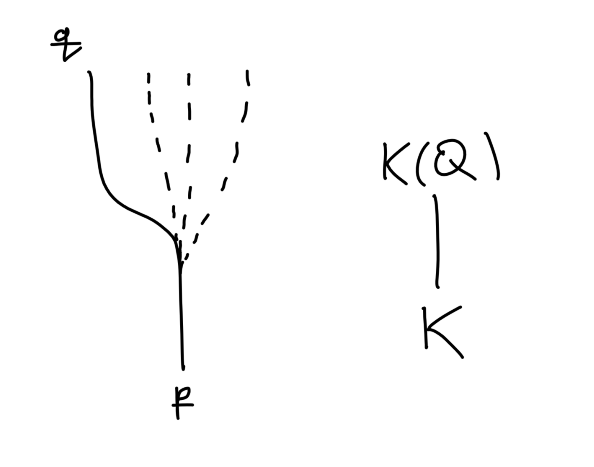
\includegraphics[scale=0.25]{lyingover}
    \end{center}
    Recall the ramification index is given by $e_{\q/\p}=|I_{\q/\p}|$, where
    \begin{equation*}
        I_{\q/\p} = \{\sigma\in\Gal(K(Q)/K)
            :\text{$\sigma(\q)=\q$ and $\sigma(t)=t\mod\q$ for all
            $t\in\O_{K(Q)}$}\}
    \end{equation*}
    is the inertia group. Hence it suffices to show that $\sigma(Q)=Q$ for all
    $\sigma\in I_{\q/\p}$, as then $\sigma$ fixes $K(Q)$ so $\sigma=\id$,
    meaning $I_{\q/\p}$ has order 1. Now for $\sigma\in I_{\q/\p}$, if
    $Q=(x_0,y_0)$ then
    \begin{equation*}
        \sigma(x_0)=x_0\mod\p,\quad\sigma(y_0)=y_0\mod\q
    \end{equation*}
    so $\overline{\sigma(Q)}=\overline Q$, and $2\sigma(Q)=\sigma(2Q)=2Q$, and
    hence $\sigma(Q)=Q\oplus T$ for some $T\in E(K)[2]$. Then
    $\overline{\sigma(Q)}=\overline Q$ implies $\overline T=\O$, and from the
    explicit list of points in $E(K)[2]$ we must have $T=\O$. Hence
    $\sigma(Q)=Q$ as required.
\end{proof}

\begin{lemma}
    Let $K$ be a number field.
    \begin{enumerate}[label=(\roman*)]
        \item If $a\in\O_K\setminus\{0\}$, and $(a)=\prod_i\p_i^{n_i}$ for
            distinct primes $\p_i$, then $K(\sqrt a)/K$ ramifies at the $\p_i$
            where $n_i$ is odd.

        \item If $S$ is a finite set of primes of $K$, then there are only
            finitely many quadratic extensions that ramify only at primes in
            $S$.
    \end{enumerate}
\end{lemma}

\begin{proof}
    Exercise.
\end{proof}

\begin{lemma}
    Let $E/K$ be an elliptic curve over a number field with
    $E(K)[2]=C_2\times C_2$. The map
    \begin{align*}
        E(K)/2E(K) &\to \{F/K:\Gal(F/K)\le C_2\times C_2\} \\
        P &\mapsto \text{$K(Q)$ where $Q\in E(\overline K)$ with $2Q=P$}
    \end{align*}
    is well-defined, and finite-to-one.
\end{lemma}

\begin{proof}
    Firstly, we check well-definedness:
    \begin{itemize}
        \item The Galois group satisfies the right condition by Lemma 25(iii).
        \item If $P=2Q=2Q'$ then $K(Q)=K(Q')$ by Lemma 25(iii).
        \item If $P'=P\oplus 2R$, and $2Q=P$, then $2Q'=P'$ for $Q'=Q\oplus R$,
            and $K(Q')\subseteq K(Q)$. We get equality by symmetry.
    \end{itemize}
    Suppose $P_1,\ldots,P_{17}\in E(K)$ have $P_i=2Q_i$, where
    $Q_i\in E(\overline K)$, and suppose all $K(Q_i)$ are equal to one field
    $F$. Write $\Gal(F/K)=\langle\sigma_1,\sigma_2\rangle\le C_2\times C_2$,
    where possibly $\sigma_i=1$. Then $\sigma_i(Q_j)=Q_j\oplus T$ with
    $T\in E(K)[2]$, and since $\#E(K)[2]^2=4^2<17$ we must have two points that
    have the same $T$ for each $\sigma_i$; without loss of generality
    \begin{align*}
        \sigma_1(Q_1) &= Q_1\oplus T \qquad \sigma_1(Q_2) = Q_2\oplus T \\
        \sigma_2(Q_1) &= Q_1\oplus T' \qquad \sigma_2(Q_2) = Q_2\oplus T'
    \end{align*}
    for some $T,T'\in E(K)[2]$. Then
    \begin{equation*}
        \sigma_1(Q_1\ominus Q_2) = Q_1\ominus Q_2 = \sigma_2(Q_1\ominus Q_2),
    \end{equation*}
    so $R=Q_1\ominus Q_2\in E(K)$. Hence $P_1\ominus P_2=2R\in 2E(K)$, so the
    map is at most 16-to-1.
\end{proof}

\begin{theorem}[Weak Mordell--Weil Theorem]
    Let $E/K$ be an elliptic curve over a number field, with
    $E(K)[2]=C_2\times C_2$. Then $E(K)/2E(K)$ is finite.
\end{theorem}

\begin{proof}
    Without loss of generality $E:y^2=(x-\alpha)(x-\beta)(x-\gamma)$ with
    $\alpha,\beta,\gamma\in\O_K$ distinct. By the previous lemma we have a
    finite-to-one map
    \begin{equation*}
        E(K)/2E(K) \to \{F/K:\Gal(F/K)\le C_2\times C_2\}.
    \end{equation*}
    Now such $F/K$ must be of the form $K(\sqrt a,\sqrt b)$ for some $a,b\in K$,
    and must only ramify at finitely many $\p$ (those satisfying
    $\p\mid2(\alpha-\beta)(\beta-\gamma)(\alpha-\gamma)$). There are only
    finitely many fields $K(\sqrt a)$, $K(\sqrt b)$ satisfying this ramification
    property by Lemma 27, and hence only finitely many such
    $K(\sqrt a,\sqrt b)$. Therefore the codomain of the map is finite, so the
    domain is finite.
\end{proof}

\begin{numberremark}
    By some algebra one can check that $E(K)/2E(K)$ is finite even if
    $E(K)[2]\ne C_2\times C_2$. (Apply the previous theorem over a splitting
    field of the cubic, and chase some diagrams.)
\end{numberremark}

\begin{theorem}[Mordell--Weil Theorem]
    Let $E/K$ be an elliptic curve over a number field. Then $E(K)$ is
    finitely generated.
\end{theorem}

\begin{proof}
    Let $F=K(\alpha,\beta,\gamma)$, where
    $E:y^2=f(x)=(x-\alpha)(x-\beta)(x-\gamma)$. Then by Theorem 23 (over number
    fields) we have
    \begin{equation*}
        E(F) \cong \Delta\times\Z^n
    \end{equation*}
    where $\Delta$ is a finite group and $n$ is possibly infinite. Then by
    Theorem 29 we have that $E(F)/2E(F)$ is finite, so $n$ must be finite.
    Since $E(K)\le E(F)$, and $E(F)$ is finitely generated, it follows that
    $E(K)$ is finitely generated. (Once can avoid using heights over number
    fields when $K=\Q$ by Remark 30.)
\end{proof}

\begin{example}
    Consider $E:y^2=x^3-x$ over $\Q$. Now
    \begin{equation*}
        E(\Q)[2]=\{\O,(0,0),(1,0),(-1,0)\}=C_2\times C_2,
    \end{equation*}
    so $E(\Q)=\Z/n\Z\times\Z/m\Z\times\Z^r$ for some $n,m$ even and $r\ge0$.
    Our proof of Theorem 29 gives a bound on $r$ as follows: For $P\in E(\Q)$,
    we have $\Q(\frac{1}{2}P)=\Q(\sqrt a,\sqrt b)$ for some $a,b$, which only
    ramifies at $p\mid 2\Disc(x^3-x)=-8$, i.e. at $p=2$. Then 2 is the only
    prime factor of $a$ and $b$, so $\Q(\frac{1}{2}P)\subseteq\Q(\sqrt2,i)$. By
    an argument as in Lemma 28, or see Exercise 3, we have an injective group
    homomorphism
    \begin{align*}
        E(\Q)/2E(\Q) &\to \Hom(\Gal(\Q(\sqrt2,i)/\Q),E(\Q)[2]) \\
        P &\mapsto (\sigma\mapsto
            \sigma({\textstyle\frac{1}{2}P})\ominus{\textstyle\frac{1}{2}P}).
    \end{align*}
    Now the Galois group of $\Q(\sqrt2,i)/\Q$ is $C_2\times C_2$, and
    $E(\Q)[2]=C_2\times C_2$, so we get
    \begin{equation*}
        E(\Q)/2E(\Q) \le C_2\times C_2\times C_2\times C_2,
    \end{equation*}
    and hence $\rk(E/\Q)=r\le2$. (In fact $r=0$, which we will be able to prove
    later.)
\end{example}

\subsection*{Exercises}

\begin{enumerate}
    \item[+1.] Let $E/\Q$ be an elliptic curve over $\Q$ given by
        \begin{align*}
            E&:\quad y^2=(x-\alpha)(x-\beta)(x-\gamma) &
            \alpha,\beta,\gamma&\in\Z.
        \end{align*}
        Find a crude\footnote{ideally logarithmic} but completely explicit bound
        on the rank of $E/\Q$ in terms of $\alpha,\beta,\gamma$.

        \begin{proof}[Solution]
            For $P\in E(\Q)/2E(\Q)$ we have
            $\Q(\frac{1}{2}P)=\Q(\sqrt a,\sqrt b)$ with $a,b\in\Z$ square-free
            and only divisible by the prime factors $p_1,\ldots,p_N$ of
            $2(\alpha-\beta)(\beta-\gamma)(\alpha-\gamma)$. This is then a
            subfield of $F=\Q(\sqrt{p_1},\ldots,\sqrt{p_N},i)$, and as in
            Exercise 3 we have an injective group homomorphism
            \begin{align*}
                E(\Q)/2E(\Q) \to \Hom(\Gal(F/\Q),E(\Q)[2])
                    &\cong \Hom(\overbrace{C_2\times\cdots\times C_2}
                        ^{\text{$N+1$ times}},C_2\times C_2) \\
                    &\cong\overbrace{C_2\times\cdots\times C_2}
                        ^{\text{$2N+2$ times}},
            \end{align*}
            implying that the rank of $E/\Q$ is at most $2N$. Now $\log p>1$
            for primes $p>2$, so taking the logarithm of a prime factorization
            we see that
            \begin{equation*}
                N\le 1 + \log\bigl(
                    |\alpha-\beta||\beta-\gamma||\alpha-\gamma|\bigr).
            \end{equation*}
            Hence
            \begin{equation*}
                \rk(E/\Q)
                    \le 2+2\log\bigl(
                        |\alpha-\beta||\beta-\gamma||\alpha-\gamma|\bigr).
            \end{equation*}
        \end{proof}

    \item[+2.] Suppose $A$ is an abelian group with $A/2A$ finite that admits a
        function $h:A\to\R_{\ge0}$ satisfying
        \begin{itemize}
            \item For every $C\in\R$ there are only finitely many $x\in A$ with
                $h(x)<C$, and
            \item $h(x+y)+h(x-y)=2h(x)+2h(y)+O(1)$, where the implied constant
                is independent of $x,y\in A$.
        \end{itemize}
        By expressing $x\in A$ as $x=a_1+2a_2+\cdots+2^na_n+2^{n+1}y$, where
        $a_i$ are fixed representatives for $A/2A$, prove that $A$ must be
        finitely generated. (This gives an elementary proof that Weak
        Mordell--Weil plus naive heights implies Mordell--Weil.)

        \begin{proof}[Solution]
            Let $C>0$ be such that $|h(x+y)+h(x-y)-2h(x)-2h(y)|\le C$ for all
            $x,y\in A$. Fix a complete set $S\subseteq A$ of representatives for
            the elements of $A/2A$. Given $x\in A$, we have some $a_0\in S$ with
            $x+a_0=2y$ for some $y\in A$, and continuing inductively we get
            $a_0,a_1,\ldots\in S$ sastifying $x+a_0+2a_1+\cdots+2^na_n=2^{n+1}y$
            for some $y\in A$ for each $n$. Now
            \begin{align*}
                h(2^{n+1}y) = h(2^ny + 2^ny)
                    &\ge 4h(2^ny) - h(0) - C \\
                    &\ge 4^{n+1}h(y) - (1 + 4 + 4^2 + \cdots + 4^n)(h(0)+C) \\
                    &\ge 4^{n+1}(h(y)-h(0)-C),
            \end{align*}
            and
            \begin{align*}
                h(2^{n+1}y) = h(2^ny+2^ny)
                    &\le 4h(2^ny) - h(0) + C \\
                    &\le 4^{n+1}h(y) + (1+4+4^2+\cdots+4^n)(C-h(0)) \\
                    &\le 4^{n+1}(h(y)-h(0)+C),
            \end{align*}
            so we get that
            \begin{equation*}
                \biggl|h(y)-\frac{h(2^{n+1}y)}{4^{n+1}}-h(0)\biggr| \le C.
            \end{equation*}
            Then
            \begin{align*}
                h(2^{n+1}y)
                    &= h(x+a_0+2a_1+\cdots+2^na_n) \\
                    &\le 2h(2^na_n) + 2h(x+a_0+2a_1+\cdots+2^{n-1}a_{n-1}) + C \\
                    &\le 2h(2^na_n) + 2^2h(2^{n-1}a_{n-1}) + \cdots
                        + 2^{n+1}h(a_0) + 2^{n+1}h(x) + (1+2+2^2+\cdots+2^n)C \\
                    &\le 2\cdot4^n\bigl(h(a_n)+C-h(0)\bigr) \\
                    &\qquad + 2^2\cdot4^{n-1}\bigl(h(a_{n-1})+C-h(0)\bigr) \\
                    &\qquad + \cdots \\
                    &\qquad + 2^n\cdot4^1\bigl(h(a_1)+C-h(0)\bigr)
                        + 2^{n+1}h(a_0) + 2^{n+1}h(x) + 2^{n+1}C \\
                    &\le 2^{2n+1}\cdot\max_{a\in S}\bigl(h(a)+C-h(0)\bigr)
                        + 2^{n+1}(h(x)+C),
            \end{align*}
            noting that $h(a_0)\le h(a_0)+C-h(0)$ since $|2h(0)-4h(0)|\le C$
            implies $h(0)\le\frac{C}{2}$. Hence
            \begin{align*}
                h(y)
                    &\le 4^{-n-1}h(2^{n+1}y) + h(0) + C \\
                    &\le 2^{-1}\cdot\max_{a\in S}\bigl(h(a)+C-h(0)\bigr)
                        + 2^{-n-1}(h(x)+C),
            \end{align*}
            so for $n$ large enough we have
            \begin{equation*}
                h(y) \le 2^{-1}\cdot\max_{a\in S}\bigl(h(a)+C-h(0)\bigr) + 1.
            \end{equation*}
            Now the set $T\subseteq A$ of $y$ satisfying this inequality is
            finite, and since $f$ is a linear combination of
            $a_0,a_1,\ldots\in S$ and $y\in T$, we see that the finite set
            $S\cup T$ generates $A$.
        \end{proof}

    \item[3.] Let $E/K$ be an elliptic curve over a number field, such that
        $E(K)[2]\cong C_2\times C_2$. Fix representatives $P_1,\ldots,P_k$ for
        $E(K)/2E(K)$, and let $Q_i\in E(\bar K)$ satisfy $2Q_i=P_i$. Show that
        the number field $F=K(Q_1,\ldots,Q_k)$ generated by the $x$- and
        $y$-coordinates of the $Q_i$ has Galois group of the form
        $G=\Gal(F/K)\cong C_2\times\cdots\times C_2$.

        Verify that for a fixed $P_i$, the map
        $f_{P_i}:\sigma\mapsto\sigma(Q_i)\ominus Q_i$ is a homomorphism from $G$
        to $E(K)[2]$. Show furthermore that the association $P_i\mapsto f_{P_i}$
        is an injective homomorphism from $E(K)/2E(K)$ to $\Hom(G,E(K)[2])$.

        Deduce that the rank of $E/K$ is at most $2n-2$, where
        $G\cong C_2\times\cdots\times C_2$ ($n$ times).

        \begin{proof}[Solution]
            For the Galois group, by Lemma 25 we have
            \begin{equation*}
                \Gal(K(Q_i)/K)\le C_2\times C_2,
            \end{equation*}
            so $K(Q_i)=K(\sqrt a,\sqrt b)$ for some $a,b\in K$. Therefore $F$ is
            given by adjoining at most $2k$ square roots to $K$, and hence $G$
            is isomorphic to a product of at most $2k$ copies of $C_2$. Now the
            maps $f_{P_i}$ are independent of the choice of $Q_i$, since if
            $2Q'_i=P_i$ then $Q_i\ominus Q'_i\in E(F)[2]$, and $E(F)[2]=E(K)[2]$
            since $E(K)[2]\cong C_2\times C_2$, so $Q_i\ominus Q'_i\in E(K)$.
            Hence for $\sigma\in G$ we have
            \begin{equation*}
                \sigma(Q_i\ominus Q'_i)\ominus(Q_i\ominus Q'_i)
                    = (Q_i\ominus Q'_i)\ominus(Q_i\ominus Q'_i)
                    = 0,
            \end{equation*}
            so $\sigma(Q_i)\ominus Q_i=\sigma(Q'_i)\ominus Q'_i$. Also
            $2f_{P_i}(\sigma)=\sigma(P_i)\ominus P_i=0$, and
            \begin{align*}
                f_{P_i}(\sigma\tau)
                    &= \sigma\tau(Q_i)\ominus Q_i \\
                    &= (\sigma\tau(Q_i)\ominus\tau(Q_i))
                        \oplus (\tau(Q_i)\ominus Q_i) \\
                    &= f_{\tau(P_i)}(\sigma) \oplus f_{P_i}(\tau) \\
                    &= f_{P_i}(\sigma) \oplus f_{P_i}(\tau),
            \end{align*}
            so $f_{P_i}(\sigma)\in E(F)[2]=E(K)[2]$ and $f_{P_i}$ is a
            homomorphism $G\to E(K)[2]$. Moreover
            \begin{align*}
                f_{P_i\oplus P_j}(\sigma)
                    &= \sigma(Q_i\oplus Q_j)\ominus Q_i\ominus Q_j \\
                    &= \sigma(Q_i)\oplus\sigma(Q_j)\ominus Q_i\ominus Q_j \\
                    &= f_{P_i}(\sigma)\oplus f_{P_j}(\sigma),
            \end{align*}
            so this gives a homomorphism $E(K)/2E(K)\to\Hom(G,E(K)[2])$. If
            $f_{P_i}=0$ then $\sigma(Q_i)=Q_i$ for all $\sigma\in G$, and hence
            $Q_i\in E(K)$, so $P_i\in 2E(K)$. Therefore this homomorphism is
            injective.

            Now by the Mordell--Weil Theorem we have $E(K)\cong\Delta\times\Z^r$
            for some finite group $\Delta$, where $r$ is the rank. Then
            \begin{equation*}
                E(K)/2E(K) \cong E(K)[2]\times C_2^r \cong C_2^{r+2},
            \end{equation*}
            and from above this is a subgroup of
            \begin{equation*}
                \Hom(G,E(K)[2]) = \Hom(C_2^n,C_2\times C_2) = C_2^{2n}.
            \end{equation*}
            Hence $r+2\le2n$, i.e. $r\le2n-2$.
        \end{proof}

    \item[4.] Let $E/K$ be an elliptic curve over a number field given by
        $y^2=x^3+ax^2+bx+c$. For $d\in K^\times$, the \emph{quadratic twist of
        $E$ by $d$} is the elliptic curve given by
        \begin{equation*}
            E_d:\quad d\cdot y^2=x^3+ax^2+bx+c.
        \end{equation*}
        Prove that $E$ and $E_d$ are isomorphic over $K(\sqrt d)$ and that (for
        $\sqrt d\notin K$)
        \begin{equation*}
            \rk E/K(\sqrt d) = \rk E/K + \rk E_d/K.
        \end{equation*}

    \item[!5.] Prove that $y^2+y=x^3+x^2+x$ has an infinite number of solutions
        over every cubic field of the form $\Q(\sqrt[3]{m})$ for $m\in\Z$.
\end{enumerate}

\section{Reduction mod $p$ and Torsion}

\begin{definition}
    For $E/K$ given by
    \begin{equation*}
        E: y^2 + a_1xy + a_3y = x^3 + a_2x^2 + a_4x + a_6 \tag{$*$}
    \end{equation*}
    the \emph{discriminant} of $E$ is
    \begin{equation*}
        \Delta_E = -b_2^2b_8 - 8b_4^3 - 27b_6^2 + 9b_2b_4b_6,
    \end{equation*}
    where
    \begin{equation*}
        b_2=a_1^2+4a_2,\,
        b_4=2a_4+a_1a_3,\,
        b_6=a_3^2+4a_6,\,
        b_8=b_2b_6-a_1a_3a_4+a_2a_3^2-a_4^2.
    \end{equation*}
\end{definition}

\begin{remark}
    If $E:y^2=f(x)$, i.e. $a_1=0=a_3$, then $\Delta_E=16\Disc(f)$. If
    $E:y^2=x^3+Ax+B$ then $\Delta_E=-16(4A^3+27B^2)$.
\end{remark}

\begin{proposition}
    \begin{enumerate}[label=(\roman*)]
        \item $E$ is non-singular iff $\Delta_E\ne0$.
        \item If $E,E'$ are isomorphic, related by a change of coordinates of
            the form
            \begin{equation*}
                y'=u^3y+sx+t,\,x'=u^2x+r,
            \end{equation*}
            then $\Delta_{E'}=u^{12}\Delta_E$.
    \end{enumerate}
\end{proposition}

\begin{proof}
    \begin{enumerate}[label=(\roman*)]
        \item See Silverman, Ch III, Prop 1.4.
        \item Computation.
    \end{enumerate}
\end{proof}

\begin{definition}
    Let $K$ be a number field (or a non-Archimedean local field), and $\p$ a
    prime of $K$. Let $E/K$ be given by ($*$). The equation is \emph{integral}
    at $\p$ if $\ord_\p(a_i)\ge0$ for all $i$. It is \emph{minimal} at $\p$ (or
    a minimal model for $E$ at $\p$) if it is integral with $\ord_\p\Delta_E$
    minimal among integral Weierstrass equations in the isomorphism class of
    $E$. The \emph{reduced curve} at $\p$ is then
    \begin{equation*}
        \tilde E/\F_\p : y^2 + \bar a_1xy + \bar a_3y
            = x^3 + \bar a_2x^2 + \bar a_4x + \bar a_6
    \end{equation*}
    for any minimal model, where $\F_\p$ is the residue field at $\p$ and
    $\bar a_i$ denotes the reduction of $a_i$ mod $\p$.
\end{definition}

\begin{remark}
    The minimal model is unique up to transformations of the form
    \begin{equation*}
        y'=u^3y+sx_t,\,x'=u^2x+r
    \end{equation*}
    where $\ord_\p$ of $u,s,t,r$ is $\ge0$ to preserve integrality and
    $\ord_\p(u)=0$ to preserve minimality by Proposition 32. This reduces to an
    isomorphism of reduced curves, so $\tilde E/\F_\p$ is well-defined up to
    isomorphism.
\end{remark}

\begin{definition}
    $E/K$ has \emph{good reduction} at $\p$ if $\tilde E/\F_\p$ is non-singular,
    and \emph{bad reduction} otherwise. We write
    \begin{equation*}
        \tilde E_\ns(\F_\p) \coloneq \tilde E(\F_\p)
            \setminus\{\text{the singular point if it exists}\}.
    \end{equation*}
\end{definition}

\begin{proposition}
    \begin{enumerate}[label=(\roman*)]
        \item $E$ has good reduction at $\p$ iff $\ord_\p(\Delta_E)=0$ for a
            minimal model.
        \item If $E$ is integral at $\p$ and $\ord_\p(\Delta_E)<12$ then $E$ is
            a minimal model.
        \item $\tilde E_\ns(\F_\p)$ is an abelian group with identity $\O$ and
            $P\oplus Q\oplus R=\O$ iff $P,Q,R$ are collinear.
    \end{enumerate}
\end{proposition}

\begin{proof}
    \begin{enumerate}[label=(\roman*)]
        \item Good reduction is equivalent to $\Delta_{\tilde E}\ne0$ by
            Proposition 32(i), which is equivalent to $\Delta_E\ne0\mod\p$ for a
            minimal model.

        \item Follows from Proposition 32(ii).

        \item See Silverman, Ch III, Prop 2.5. (It is clear if $\tilde E$ is
            non-singular.)
    \end{enumerate}
\end{proof}

\begin{remark}
    We have the following taxonomy of reduction types:
    \begin{itemize}
        \item Good reduction
            $\iff$ $\tilde E$ is non-singular.
        \item Split multiplicative reduction
            $\iff$ $\tilde E_\ns(\F_\p)\cong\F_\p^\times$.
        \item Non-split multiplicative reduction
            $\iff$
            $\tilde E_\ns(\F_\p)\cong\F_{q^2}^\times/\F_q^\times\cong C_{q+1}$
            where $q=|\F_\p|$.
        \item Additive reduction
            $\iff$ $\tilde E_\ns(\F_\p)\cong(\F_\p,+)$.
    \end{itemize}
    The last three are classified as bad reduction, and the first three are
    classified as ``semistable'' reduction. When $\p\nmid2$ there is a minimal
    model of the form $E:y^2=f(x)$, and then we have the following
    characterizations:
    \begin{itemize}
        \item Good reduction $\iff$ $f(x)$ has distinct roots mod $\p$.
        \item Multiplicative reduction $\iff$ $f(x)$ has a double root mod $\p$.
            Here $\tilde E$ can be written as $y^2=x^2(x+\eta)$, and
            $\eta\in(\F_\p^\times)^2$ $\iff$ the reduction is split
            multiplicative. (This is equivalent to the slopes of the two tangent
            lines being defined over $\F_\p$.) The isomorphism
            \begin{equation*}
                \tilde E_\ns(\F_\p)\cong\F_\p^\times
                    \quad\text{or}\quad\F_{q^2}^\times/\F_q^\times
            \end{equation*}
            is given by $(x,y)\mapsto-y/x$.
        \item Additive reduction $\iff$ $f(x)$ has a triple root mod $\p$. Here
            the isomorphism
            \begin{equation*}
                \tilde E_\ns(\F_\p)\cong(\F_\p,+)
            \end{equation*}
            is given by $(x,y)\mapsto-y/x$.
    \end{itemize}
\end{remark}

\begin{example}
    $E:y^2=x^3-3\cdot5^4x-3\cdot5^6$ has $\Delta_E=-2^4\cdot3^3\cdot5^{13}$, and
    is integral but not minimal at 5; we can take
    \begin{equation*}
        x=5^2x',\,y=5^3y'
    \end{equation*}
    to get
    \begin{equation*}
        E':y'^2=x'^3-3x'-3
    \end{equation*}
    which is integral, and has $\Delta_{E'}=-2^4\cdot3^3\cdot5$, so it is
    minimal by Proposition 33(ii). The reduced curve is then
    \begin{equation*}
        \tilde E:y^2=x^3+2x+2 = (x-1)^2(x+2) / \F_5
    \end{equation*}
    which is isomorphic to $y^2=x^2(x+3)$, and hence has multiplicative
    reduction which is non-split as $3\notin(\F_5^\times)^2$. The points are
    \begin{equation*}
        \tilde E(\F_5) = \{\text{the singular point $(1,0)$}\}
            \cup\{(2,\pm2),(3,0),(4,\pm2),\O\},
    \end{equation*}
    and we see $\tilde E_\ns(\F_5)\cong C_6$.
\end{example}

\begin{remark}
    We have $\Q\subseteq\Q_p$, so $E(\Q)\subseteq E(\Q_p)$. In this and the
    following section we will describe $E(\Q_p)$.
\end{remark}

\begin{definition}
    Let $E/K$ be an elliptic curve over a non-Archimedean local field (e.g.
    $\Q_p$). Then
    \begin{align*}
        E_0(K) &\coloneq \{P\in E(K)
            :\text{$P$ reduces to a point in $\tilde E_\ns(\F_\p)$}\} \\
        E_1(K) &\coloneq \{P\in E(K)
            :\text{$P$ reduces to $\O\in\tilde E_\ns(\F_\p)$}\}.
    \end{align*}
\end{definition}

\begin{lemma}
    \begin{enumerate}[label=(\roman*)]
        \item $E_1(K)\le E_0(K)\le E(K)$ are subgroups.
        \item The reduction mod $\p$ map $P\mapsto\tilde P$ is a homomorphism
            $E_0(K)\to\tilde E_\ns(\F_\p)$.
    \end{enumerate}
\end{lemma}

\begin{proof}
    The inclusions are clear, $E_0(K)$ is a subgroup since $\tilde E_\ns(\F_\p)$
    is a group and the reduction map respects the group structure by Proposition
    33(iii). Then $E_1(K)$ is also a subgroup, being the kernel of the reduction
    map.
\end{proof}

\begin{theorem}
    Let $E/K$ be an elliptic curve over a non-Archimedean local field. Let
    $n=\ord_\p\Delta_{E'}$ for a minimal model $E'$ of $E$. Then $E(K)/E_0(K)$
    is finite, and
    \begin{enumerate}[label=(\roman*)]
        \item $E(K)/E_0(K)=1$ if $E/K$ has good reduction.
        \item $E(K)/E_0(K)\cong\Z/n\Z$ if $E/K$ has split multiplicative
            reduction.
        \item We have
            \begin{equation*}
                E(K)/E_0(K)\cong \begin{dcases*}
                    1 & $n$ odd \\
                    \Z/2\Z & $n$ even.
                \end{dcases*}
            \end{equation*}
            if $E/K$ has non-split multiplicative reduction.
        \item $|E(K)/E_0(K)|\le4$ if $E/K$ has additive reduction.
    \end{enumerate}
\end{theorem}

\begin{proof}
    (i) is clear. For the rest, see Silverman's ``Advanced Topics...''.
\end{proof}

\begin{remark}
    The order $|E(K)/E_0(K)|$ is called the \emph{local Tamagawa number},
    usually written $c_\p$ or $c(E/K)$. The group $E(K)/E_0(K)$ and its order
    $c_\p$ are fully determined by ``Tate's algorithm''.
\end{remark}

\begin{theorem}
    Let $E/K$ be ane elliptic curve over a non-Archimedean local field, given by
    a minimal Weierstrass equation. The reduction mod $\p$ map induces an
    isomorphism
    \begin{equation*}
        E_0(K)/E_1(K) \xrightarrow\sim \tilde E_\ns(\F_\p).
    \end{equation*}
\end{theorem}

\begin{proof}
    By Lemma 34 this is a homomorphism, which is injective by the definition of
    $E_1(K)$, so it suffices to prove surjectivity. Write the equation for $E$
    as
    \begin{equation*}
        E:g(x,y)=0,\quad g(x,y)=y^2+a_1xy+a_3y-x^3-a_2x^2-a_4x-a_6,
    \end{equation*}
    with $a_i\in\O_K$. If $P_0=(x_0,y_0)\in\tilde E_\ns(\F_\p)$, we have either
    $\pdv{g}{x}|_{P_0}\ne0$ or $\pdv{g}{y}|_{P_0}\ne0$. By symmetry, assume
    $\pdv{g}{y}|_{P_0}\ne0$, and pick some $x\in\O_K$ with $\bar x=x_0$. Then by
    Hensel's lemma, we can solve $g(x,y)=0$ for $y$ subject to $\bar y=y_0$.
\end{proof}

\begin{theorem}
    Let $E/\Q_p$ be an elliptic curve. Then $E_1(\Q_p)$ contains no non-trivial
    points of finite order, except possibly points of order 2 if $p=2$.
\end{theorem}

\begin{proof}
    This will be proved in the next section.
\end{proof}

\begin{corollary}
    Let $E/\Q$ be an elliptic curve, with $p$ a prime of good reduction. Then
    the reduction map
    \begin{equation*}
        E(\Q)_\tors \to \tilde E(\F_p)
    \end{equation*}
    is injective, except possibly if $p=2$ where it may have kernel contained in
    $E(\Q)[2]$.
\end{corollary}

\begin{proof}
    The kernel is $\bigl(E(\Q)\cap E_1(\Q_p)\bigr)_\tors$. Now apply Theorem 37.
\end{proof}

\begin{corollary}[Nagell--Lutz Theorem]
    Let $E/\Q$ be an elliptic curve given by
    \begin{equation*}
        y^2 = x^3 + Ax + B,\quad A,B\in\Z.
    \end{equation*}
    If $P=(x_0,y_0)$ is a non-trivial point of finite order, then
    \begin{enumerate}[label=(\roman*)]
        \item $x_0,y_0\in\Z$, and
        \item $y_0=0$ or $y_0^2$ divides $4A^3+27B^2$.
    \end{enumerate}
\end{corollary}

\begin{proof}
    \begin{enumerate}[label=(\roman*)]
        \item If $P$ has order 2 then $y_0=0$, and $x_0$ is a root of $x^3+Ax+B$,
            and hence is an integer by the rational root theorem. Now suppose
            $P$ has order greater than 2. Let $p$ be a prime, with $E'$ a
            minimal model at $p$, and let $P'=(x_1,y_1)$ be the corresponding
            point on $E'$. By Theorem 37 we have $P'\notin E_1(\Q_p)$, so $P'$
            does not reduce to $\O$, and hence $x_1,y_1\in\Z_p$ are $p$-adic
            integers. The change of coordinates
            \begin{equation*}
                y'=u^3y+sx+t,\,x'=u^2x+r
            \end{equation*}
            with some algebra then gives that $x_0,y_0\in\Z_p$. Since
            $x_0,y_0\in\Q$ it follows that $x_0,y_0\in\Z$.

        \item If $y_0\ne0$ we may check that
            \begin{equation*}
                y_0^2(4f(x_0)x_1-g(x_0)) = 4A^3 + 27B^2,
            \end{equation*}
            where $f(x)=3x^2+4A$, $g(x)=3x^2-5Ax-27B$, and $x_1$ is the
            $x$-coordinate of $2P$, which is an integer by (i).
    \end{enumerate}
\end{proof}

\begin{remark}
    Corollaries 38 and 39 give practical ways to determine $E(\Q)_\tors$; either
    compute $\tilde E(\F_p)$ for a few primes to bound $E(\Q)_\tors$, or
    factorize $4A^3+27B^2$ for possible $y_0$ and solve for $x_0$.
\end{remark}

\subsection*{Exercises}

\begin{enumerate}
    \item[+1.] Let $E/\Q$ be the elliptic curve given by $y^2+y=x^3-x^2$. Show
        that $E$ has discriminant $-11$ and that it has good reduction at 2 and
        split multiplicative reduction at 11. Prove that $E(\Q)_\tors\cong C_5$.

        (\textit{Recall from Exercise Sheet 1 that $(0,0)\in E(\Q)$ has order
        5.})

    \item[+2.] Show that $y^2+y=x^3-x$ has infinitely many rational solutions.

    \item[3.] Show that if $E$ does not have multiplicative reduction at 2, 3 or
        5, then $|E(\Q)_\tors|\le6$.

    \item[4.] Suppose the elliptic curve $E:y^2+a_1xy+a_3y=x^3+a_2x^2+a_4x+a_6$,
        with $a_i\in\Q$ is integral at $p$. Check that a substitution of the
        form $x=u^2x'+r$, $y=u^3y'+su^2x'+t$, for $r,s,t\in\Z$ and
        $u\in\Q^\times$ with $\ord_pu=0$, yields another equation $E'$ that is
        integral at $p$ and with $\ord_p\Delta_E=\ord_p\Delta_{E'}$.

        Show also that there must be a substitution of this form with
        $r,s,t\in\Z$ and $u$ purely a power of $p$, that will make the equation
        minimal at $p$.

        Prove that every elliptic curve over $\Q$ has a model which is minimal
        at all primes simultaneously. (This is called a \emph{global minimal
        model}. What goes wrong over larger number fields?)

    \item[!5.] Prove that there is a constant $C\in\R$ such that for every
        elliptic curve $E/\Q$,
        \begin{equation*}
            \Delta_E<C\cdot P_E^{13},
        \end{equation*}
        where $\Delta_E$ is the minimal discriminant of $E$ and $P_E$ is the
        product of the primes at which $E$ has bad reduction.
\end{enumerate}

\end{document}
